%============================================================
%  TESIS DE GRADO EN INGENIERÍA ELECTRÓNICA / TELECOMUNICACIONES
%  Título provisional: Procesamiento de señales para radar de
%  penetración terrestre (GPR) tipo FMCW
%============================================================

\documentclass[12pt, a4paper, twoside]{report}

%------------------------------------------------------------
% PAQUETES
%------------------------------------------------------------
\usepackage[utf8]{inputenc}
\usepackage[T1]{fontenc}
\usepackage[spanish]{babel}
\usepackage{lmodern}

% Márgenes (IRAM / normas universitarias argentinas)
\usepackage[
  top=2.5cm, bottom=2.5cm,
  inner=3.0cm, outer=2.0cm
]{geometry}

% Matemáticas
\usepackage{amsmath, amssymb, amsfonts}
\usepackage{bm}           % vectores en negrita

% Tablas
\usepackage{booktabs}
\usepackage{array}
\usepackage{longtable}
\usepackage{multirow}

% Figuras
\usepackage{graphicx}
\usepackage{float}
\usepackage{caption}
\usepackage{subcaption}
\usepackage{tikz}
\usetikzlibrary{arrows.meta, positioning, fit}

% Colores y código fuente
\usepackage{xcolor}
\usepackage{listings}

% Hipervínculos (debe ir casi al final)
\usepackage[
  colorlinks=true,
  linkcolor=blue!60!black,
  citecolor=green!50!black,
  urlcolor=blue!70!black
]{hyperref}

% Bibliografía
\usepackage[
  backend=biber,
  style=ieee,
  sorting=none
]{biblatex}
\addbibresource{referencias.bib}

% Encabezados y pies de página
\usepackage{fancyhdr}
\pagestyle{fancy}
\fancyhf{}
\fancyhead[LE,RO]{\thepage}
\fancyhead[RE]{\nouppercase{\leftmark}}
\fancyhead[LO]{\nouppercase{\rightmark}}
\renewcommand{\headrulewidth}{0.4pt}

% Espaciado
\usepackage{setspace}
\onehalfspacing

% Párrafos sin sangría, con espacio entre ellos
\setlength{\parindent}{0pt}
\setlength{\parskip}{6pt}

%------------------------------------------------------------
% DATOS DE LA TESIS  (modificar según corresponda)
%------------------------------------------------------------
\newcommand{\TituloTesis}{Procesamiento de Señales para Radar de
Penetración Terrestre (GPR)}
\newcommand{\Autor}{[Nombre del Autor]}
\newcommand{\Director}{[Nombre del Director]}
\newcommand{\Institucion}{[Universidad]}
\newcommand{\Facultad}{[Facultad / Departamento]}
\newcommand{\Carrera}{Ingeniería Electrónica / Telecomunicaciones}
\newcommand{\AnioTesis}{2025}

%------------------------------------------------------------
% CONFIGURACIÓN DE LISTINGS (código MATLAB/Python)
%------------------------------------------------------------
\lstset{
  basicstyle=\ttfamily\small,
  keywordstyle=\color{blue}\bfseries,
  commentstyle=\color{gray}\itshape,
  stringstyle=\color{orange!70!black},
  numbers=left,
  numberstyle=\tiny\color{gray},
  stepnumber=1,
  numbersep=8pt,
  frame=single,
  rulecolor=\color{black!30},
  breaklines=true,
  captionpos=b,
  tabsize=4
}

%============================================================
\begin{document}

%============================================================
%  PORTADA
%============================================================
\begin{titlepage}
  \centering
  \vspace*{1.5cm}

  {\Large \textbf{\Institucion}}\\[0.4cm]
  {\large \Facultad}\\[0.4cm]
  {\large \Carrera}

  \vspace{1.5cm}
  \rule{\linewidth}{0.5pt}\\[0.4cm]
  {\LARGE \textbf{\TituloTesis}}\\[0.2cm]
  \rule{\linewidth}{0.5pt}

  \vspace{1.5cm}
  {\large Trabajo Final de Grado}

  \vfill

  \begin{tabular}{rl}
    \textbf{Autor:}    & \Autor    \\[4pt]
    \textbf{Director:} & \Director \\
  \end{tabular}

  \vspace{1.5cm}
  {\large \AnioTesis}
\end{titlepage}

%============================================================
%  PÁGINAS PRELIMINARES
%============================================================
\pagenumbering{roman}

%------------------------------------------------------------
% Índices
%------------------------------------------------------------
\tableofcontents
\clearpage
\listoffigures
\clearpage
\listoftables
\clearpage

%============================================================
%  CUERPO PRINCIPAL
%============================================================
\pagenumbering{arabic}

%============================================================
\chapter{Fundamentos Teóricos}
\label{ch:fundamentos}
%============================================================

\section{Principios de operación del GPR}

El GPR es un sistema de teledetección electromagnética que emite
energía de radiofrecuencia hacia el subsuelo y registra las reflexiones
producidas en las interfases entre materiales de distinta permitividad
eléctrica $\varepsilon_r$. La profundidad de penetración y la resolución
en rango dependen de la frecuencia central y el ancho de banda del sistema.

\subsection{Configuraciones de operación}

Los radares GPR pueden clasificarse según su forma de modulación:

\begin{itemize}
  \item \textbf{GPR de impulso:} emite pulsos muy cortos de banda ultra
    ancha (UWB). Resolución en rango determinada por el ancho del
    pulso.
  \item \textbf{SFCW} (\textit{Stepped-Frequency Continuous-Wave}): barre
    el espectro en pasos discretos de frecuencia.
  \item \textbf{FMCW} (\textit{Frequency-Modulated Continuous-Wave}): barre
    el espectro de forma continua y lineal (chirp).
\end{itemize}

\section{Sistema FMCW: parámetros fundamentales}
\label{sec:parametros_fmcw}

Un sistema FMCW emite una señal cuya frecuencia instantánea varía
linealmente en el tiempo, denominada \textit{chirp}. Los parámetros
principales se resumen en la Tabla~\ref{tab:parametros}.

\begin{table}[H]
  \centering
  \caption{Parámetros principales del sistema FMCW GPR
  (valores de referencia tomados de~\cite{Huang2022}).}
  \label{tab:parametros}
  \begin{tabular}{clll}
    \toprule
    \textbf{Símbolo} & \textbf{Nombre} & \textbf{Definición} & \textbf{Valor de ref.}\\
    \midrule
    $T_c$  & Período del chirp     & —                      & $0{,}3\,\text{s}$          \\
    $B$    & Ancho de banda        & $f_\text{max} - f_\text{min}$ & $1\,\text{GHz}$      \\
    $f_c$  & Frecuencia central    & $(f_\text{max}+f_\text{min})/2$ & $1{,}5\,\text{GHz}$\\
    $S$    & Tasa de barrido       & $B/T_c$ (diente de sierra) & $3{,}33\,\text{GHz/s}$ \\
    $c$    & Velocidad de la luz   & —                      & $3\times10^8\,\text{m/s}$  \\
    $\varepsilon_r$ & Permitividad relativa & — & Dep.\ del material        \\
    \bottomrule
  \end{tabular}
\end{table}

La frecuencia instantánea transmitida es:

\begin{equation}
  f_\text{tx}(t) = f_c - \frac{B}{2} + S\,t,
  \qquad 0 \leq t \leq T_c.
  \label{eq:f_tx}
\end{equation}

\paragraph{Advertencia sobre la convención de $S$ y $T_c$.}
La ecuación~\eqref{eq:f_tx} y la Tabla~\ref{tab:parametros} corresponden a un
chirp de \textbf{diente de sierra}, que es la modulación del sistema de
referencia~\cite{Huang2022}: la frecuencia recorre todo el ancho de banda $B$
en el período completo $T_c$, y por lo tanto $S = B/T_c$.

El sistema desarrollado en esta tesis usa en cambio modulación
\textbf{triangular}, y mantiene a $T_c$ como el \emph{período completo} de la
triangular. Cada rampa dura entonces $T_c/2$ y la tasa de barrido es el doble:
$S = 2B/T_c$ (se deduce en la ecuación~\eqref{eq:sweep_rate}). \textbf{De acá en
adelante rige esa convención}, y todas las expresiones del
Capítulo~\ref{ch:senal_if} están escritas con ella. Es la fuente de error más
fácil al comparar contra la bibliografía: un factor 2 en la frecuencia de batido
y en el espesor estimado.

\section{Propagación en medios estratificados}

La velocidad de propagación de la onda electromagnética en un medio
con permitividad relativa $\varepsilon_r$ es:

\begin{equation}
  v = \frac{c}{\sqrt{\varepsilon_r}}.
  \label{eq:velocidad_medio}
\end{equation}

Para los materiales de mayor interés práctico se indican valores
típicos de $\varepsilon_r$ en la Tabla~\ref{tab:epsilon}.

\begin{table}[H]
  \centering
  \caption{Permitividad relativa de materiales constructivos típicos.}
  \label{tab:epsilon}
  \begin{tabular}{lcc}
    \toprule
    \textbf{Material}    & $\boldsymbol{\varepsilon_r}$ & $\boldsymbol{\sqrt{\varepsilon_r}}$ \\
    \midrule
    Aire                 & $1{,}0$       & $1{,}000$ \\
    Asfalto seco         & $4 - 7$       & $2{,}00 - 2{,}65$ \\
    Asfalto húmedo       & $6 - 9$       & $2{,}45 - 3{,}00$ \\
    Concreto             & $8 - 12$      & $2{,}83 - 3{,}46$ \\
    Pared (cemento)      & $5 - 6$       & $2{,}24 - 2{,}45$ \\
    Hielo                & $3{,}2$       & $1{,}79$ \\
    \bottomrule
  \end{tabular}
\end{table}

%============================================================
\chapter{Señal IF y Frecuencia de Batido}
\label{ch:senal_if}
%============================================================

\section{Señal transmitida y frecuencia instantánea}
\label{sec:fi_inst}

La señal transmitida es un coseno cuya fase instantánea $\phi(t)$
está determinada por la frecuencia instantánea $f(t)$:

\begin{equation}
  s_\text{tx}(t) = A\cos\!\bigl(\phi(t)\bigr),
  \qquad
  \phi(t) = 2\pi\int_0^t f(t')\,dt'.
  \label{eq:stx_general}
\end{equation}

En el radar FMCW con modulación triangular, la frecuencia
instantánea varía linealmente en forma de diente triangular: asciende
de $f_c - B/2$ a $f_c + B/2$ durante el primer semiperíodo
$T_c/2$, y desciende simétricamente durante el segundo. La tasa de
barrido (en módulo) es la misma en ambas ramas:

\begin{equation}
  S \;=\; \frac{B}{T_c/2} \;=\; \frac{2B}{T_c}.
  \label{eq:sweep_rate}
\end{equation}

La frecuencia instantánea es, por tanto:

\begin{equation}
  f(t) =
  \begin{cases}
    \displaystyle f_c - \frac{B}{2} + S\,t,
    & 0 \leq t \leq \dfrac{T_c}{2}, \\[10pt]
    \displaystyle f_c + \frac{B}{2} - S\!\left(t - \frac{T_c}{2}\right),
    & \dfrac{T_c}{2} < t \leq T_c.
  \end{cases}
  \label{eq:f_inst}
\end{equation}

Dado que las dos ramas son simétricas y producen la misma frecuencia
de batido (véase la Sección~\ref{sec:beat_freq}), el desarrollo
analítico se realiza sobre la \textbf{rampa ascendente}
($0 \leq t \leq T_c/2$); los resultados son directamente aplicables
a la rampa descendente por simetría.

Sustituyendo la rama ascendente de~\eqref{eq:f_inst}
en~\eqref{eq:stx_general}:

\begin{equation}
  \phi(t) = 2\pi\int_0^t \!\left(f_c - \frac{B}{2} + S\,t'\right)dt'
  = 2\pi\left[\left(f_c - \frac{B}{2}\right)t + \frac{S}{2}\,t^2\right].
\end{equation}

La señal transmitida durante la rampa ascendente es, entonces:

\begin{equation}
  \boxed{
    s_\text{tx}(t) = A\cos\!\left(
      2\pi\left[\left(f_c - \frac{B}{2}\right)t + \frac{B}{T_c}\,t^2\right]
    \right),
    \qquad 0 \leq t \leq \frac{T_c}{2}.
  }
  \label{eq:stx}
\end{equation}

Esta expresión muestra que la señal es un chirp lineal que parte
de la frecuencia $f_c - B/2$ y llega a $f_c + B/2$ al cabo del
semiperíodo.

\section{Señal recibida}
\label{sec:senal_rx}

Un obstáculo ubicado a distancia $d$ del radar produce una señal
reflejada con retardo $\tau_d = 2d/c$, donde $c$ es la velocidad de
propagación en el medio. Durante la rampa ascendente, la señal
recibida es una réplica de~\eqref{eq:stx} retrasada $\tau_d$ segundos.
Definiendo $\tau_d \ll T_c/2$ (condición habitualmente satisfecha en
GPR), la señal recibida válida en el intervalo
$\tau_d \leq t \leq T_c/2$ es:

\begin{equation}
  \Gamma(t) = A' \cos\!\left(
    2\pi\left[\left(f_c - \frac{B}{2}\right)(t-\tau_d)
    + \frac{B}{T_c}(t-\tau_d)^2\right] - \theta
  \right),
  \label{eq:gamma}
\end{equation}

donde $A'$ absorbe la atenuación de propagación y $\theta$ una fase
inicial arbitraria. La señal~\eqref{eq:gamma} es estructuralmente
idéntica a $s_\text{tx}(t)$, pero con el argumento temporal
desplazado por $\tau_d = 2d/c$.

\section{Proceso de desrampa (\textit{dechirp} / \textit{mixing})}
\label{sec:mixing}

Al multiplicar $s_\text{tx}(t)$ (ec.~\eqref{eq:stx}) por $\Gamma(t)$
(ec.~\eqref{eq:gamma}) y aplicar un filtro pasa-bajos, se obtiene la
\textbf{señal IF} o señal de batido. Usando la identidad trigonométrica:

\begin{equation}
  \cos x \cdot \cos y = \tfrac{1}{2}\bigl[\cos(x - y) + \cos(x + y)\bigr],
\end{equation}

el producto $s_\text{tx}(t)\cdot\Gamma(t)$ genera dos términos: uno de
diferencia de fases (baja frecuencia, conservado por el filtro
pasa-bajos) y uno de suma (alta frecuencia, eliminado). Definiendo
$\tau_d = 2d/c$ por brevedad, las fases instantáneas son:

\begin{align}
  \psi_\text{tx}(t) &= 2\pi\left[\left(f_c-\tfrac{B}{2}\right)t
  + \tfrac{B}{T_c}\,t^2\right], \\
  \psi_\text{rx}(t) &= 2\pi\left[\left(f_c-\tfrac{B}{2}\right)(t-\tau_d)
  + \tfrac{B}{T_c}(t-\tau_d)^2\right] - \theta.
\end{align}

El término de diferencia, tras el filtrado pasa-bajos, es:

\begin{equation}
  x'(t) = A^*\cos\!\bigl[\psi_\text{tx}(t) - \psi_\text{rx}(t)\bigr].
\end{equation}

Calculando la diferencia de fases:

\begin{align}
  \psi_\text{tx} - \psi_\text{rx}
  &= 2\pi\left(f_c - \frac{B}{2}\right)\tau_d
  + \frac{2\pi B}{T_c}\!\left[t^2 - (t-\tau_d)^2\right] + \theta.
\end{align}

Desarrollando el binomio $(t-\tau_d)^2 = t^2 - 2\tau_d t + \tau_d^2$:

\begin{equation}
  t^2 - (t-\tau_d)^2 = 2\tau_d\,t - \tau_d^2,
\end{equation}

con lo que:

\begin{align}
  \psi_\text{tx} - \psi_\text{rx}
  &= 2\pi\left[\left(f_c-\frac{B}{2}\right)\tau_d
    + \frac{2B}{T_c}\tau_d\,t
  - \frac{B}{T_c}\tau_d^2\right] + \theta.
  \label{eq:diff_phase}
\end{align}

La señal IF resultante es, por tanto:

\begin{equation}
  x'(t) = A^*\cos\!\left[
    2\pi\frac{2B}{T_c}\tau_d\,t
    + 2\pi\!\left(f_c-\frac{B}{2}\right)\!\tau_d
    - \frac{2\pi B}{T_c}\tau_d^2 - \theta
  \right],
  \quad \tau_d \leq t \leq \frac{T_c}{2}.
  \label{eq:xIF}
\end{equation}

\section{Frecuencia de batido}
\label{sec:beat_freq}

Identificando en~\eqref{eq:xIF} el coeficiente lineal en $t$,
la \textbf{frecuencia de batido} de la rampa ascendente es:

\begin{equation}
  f_b^+ = \frac{2B}{T_c}\,\tau_d = \frac{2B}{T_c}\cdot\frac{2d}{c}
  = \frac{4Bd}{c\,T_c}.
  \label{eq:fb_up}
\end{equation}

Los términos restantes de~\eqref{eq:xIF} son puramente de fase
(constantes respecto de $t$); agrupándolos en $\varphi^*$:

\begin{equation}
  \varphi^* = 2\pi\!\left(f_c - \frac{B}{2}\right)\!\tau_d
  - \frac{2\pi B}{T_c}\tau_d^2 + \theta,
\end{equation}

la señal IF adopta la forma compacta de tono sinusoidal puro:

\begin{equation}
  \boxed{
    x'(t) = A^*\cos\!\bigl(2\pi f_b^+\, t + \varphi^*\bigr),
    \qquad \tau_d \leq t \leq \frac{T_c}{2}.
  }
  \label{eq:xIF_compact}
\end{equation}

\subsection*{Rampa descendente: simetría del resultado}

Durante la rampa descendente la tasa de barrido es $-S = -2B/T_c$.
Repitiendo el mismo desarrollo con $f(t) = f_c + B/2 - S(t-T_c/2)$
se obtiene una frecuencia de batido $f_b^- = f_b^+$ (el signo de $S$
cancela con el cambio de signo del retardo relativo). En consecuencia,
\textbf{ambas ramas producen la misma frecuencia de batido en módulo}:

\begin{equation}
  \boxed{
    f^* \;=\; f_b^+ \;=\; f_b^- \;=\; \frac{4Bd}{c\,T_c}.
  }
  \label{eq:beat_freq}
\end{equation}

Cada semiperíodo puede procesarse de forma independiente con
la FFT, y los espectros resultantes son equivalentes.
En la práctica se puede promediar la magnitud de ambos para
mejorar la relación señal a ruido.
El signo negativo del coeficiente lineal en la rampa descendente no altera la frecuencia observable: para una señal real, $\cos(-2\pi f_0 t)$ y $\cos(2\pi f_0 t)$ producen el mismo pico espectral en $\lvert f_0 \rvert$. La diferencia de signo se absorbe en la fase inicial y no afecta la estimación de distancia.

\section{Prueba de validación con reflector metálico}
\label{sec:prueba_metalica}

Antes de abordar escenarios con múltiples capas y materiales de
permitividad desconocida, resulta conveniente realizar una prueba
de validación en condiciones controladas. El caso más simple consiste
en apuntar el radar a una \textbf{plancha metálica plana} ubicada a
una distancia $d$ conocida en aire libre.

\subsection{Por qué es un caso ideal}

Un metal conductor actúa como un reflector casi perfecto: su
coeficiente de reflexión en módulo es $|\Gamma| \approx 1$. Esto
implica tres ventajas para la validación:

\begin{enumerate}
  \item \textbf{Reflexión única.} Solo existe una interfase
    (aire--metal), por lo que la señal IF contiene una única
    frecuencia de batido $f^*$, sin ambigüedad.
  \item \textbf{Sin incertidumbre en $\varepsilon_r$.} La propagación
    ocurre íntegramente en aire ($\varepsilon_r = 1$,
    $c_\text{medio} = c$), eliminando una variable desconocida.
  \item \textbf{Resultado verificable \textit{a priori}.} Conocida $d$,
    el valor teórico de $f^*$ se puede calcular antes de la medición
    y comparar directamente con el pico observado en el espectro.
\end{enumerate}

\subsection{Predicción teórica de $f^*$}

En aire libre ($\varepsilon_r = 1$), la ecuación~\eqref{eq:beat_freq}
se simplifica a:

\begin{equation}
  f^* = \frac{4Bd}{c\,T_c},
  \label{eq:beat_freq_aire}
\end{equation}

e inversamente, la distancia estimada a partir de la frecuencia
medida $\hat{f}^*$ es:

\begin{equation}
  \hat{d} = \frac{c\,T_c\,\hat{f}^*}{4B}.
  \label{eq:d_estimada}
\end{equation}

El error absoluto de distancia queda:

\begin{equation}
  \Delta d = \left|\hat{d} - d\right|.
  \label{eq:error_d}
\end{equation}

\subsection{Parámetros del sistema y frecuencias esperadas}

El sistema opera con $B = 1\,\text{GHz}$ (barrido de $1\,\text{GHz}$ a
$2\,\text{GHz}$). El período de la triangular $T_c$, en cambio, \textbf{no es un
valor fijo del sistema}: es un parámetro de la medición, que se ajusta según la
profundidad de interés y las condiciones del ensayo, y que el firmware configura
por consola. La constante del radar es, por lo tanto, función de $T_c$:

\begin{equation}
  \frac{f^*}{d} = \frac{4B}{c\,T_c}
  = \frac{4\times10^9}{3\times10^8\;T_c}
  = \frac{13{,}3}{T_c}\ \ \text{[Hz/m]},
  \qquad T_c\ \text{en segundos}.
  \label{eq:constante_radar}
\end{equation}

La Tabla~\ref{tab:prueba_metalica} evalúa esa constante para tres valores
representativos de $T_c$ y para distancias típicas de un banco de prueba en
interiores.

\begin{table}[H]
  \centering
  \caption{Frecuencia de batido teórica $f^*$ en aire libre
    ($B = 1\,\text{GHz}$) para tres períodos de triangular. Recordar que
  $T_c$ es el período completo: cada rampa dura $T_c/2$.}
  \label{tab:prueba_metalica}
  \begin{tabular}{cccc}
    \toprule
    & \multicolumn{3}{c}{$f^*\,\textnormal{[Hz]}$} \\
    \cmidrule(l){2-4}
    $d\,\textnormal{[m]}$ & $T_c = 10\,\text{ms}$ & $T_c = 50\,\text{ms}$
    & $T_c = 300\,\text{ms}$ \\
    \midrule
    0{,}10 &  133 &  27 &  4{,}4 \\
    0{,}20 &  267 &  53 &  8{,}9 \\
    0{,}50 &  667 & 133 & 22{,}2 \\
    1{,}00 & 1333 & 267 & 44{,}4 \\
    \bottomrule
  \end{tabular}
\end{table}

Dos condiciones acotan la elección de $T_c$, una por arriba y otra por abajo:

\begin{itemize}
  \item \textbf{Barridos lentos ($T_c$ grande).} La señal de batido tiene que
    quedar por encima del pasa-altos no desactivable del ADC PCM1808, cuyo corte
    combinado es de $\approx 1{,}2\,\text{Hz}$. Ya con
    $T_c = 300\,\text{ms}$ un blanco a $0{,}10\,\text{m}$ cae en
    $4{,}4\,\text{Hz}$, sobre el faldón del filtro; con barridos de segundos el
    blanco cercano se pierde adentro del filtro y su fase queda distorsionada.
  \item \textbf{Barridos rápidos ($T_c$ chico).} Hace falta $f_s > 2f^*$
    (Nyquist). Con $T_c = 10\,\text{ms}$ y $f_s = 48\,\text{kHz}$ el alcance
    máximo sin \textit{aliasing} es de $18\,\text{m}$, muy por encima de lo
    útil: el límite efectivo lo impone la cantidad de escalones que alcanza a
    escribir el DAC durante la rampa, no el muestreo.
\end{itemize}

\subsection{Procedimiento experimental propuesto}

\begin{enumerate}
  \item Colocar la antena del radar frente a la plancha metálica,
    con separación $d$ medida con cinta métrica.
  \item Verificar que no haya otros objetos reflectores en el campo
    de visión del radar (paredes, mesas, superficies metálicas
    laterales) para evitar reflexiones espurias.
  \item Adquirir la señal IF durante al menos un período completo de la
    triangular $T_c$, muestreando a $f_s > 2f^*$.
  \item Calcular $f^*_\text{teo}$ con la
    ecuación~\eqref{eq:beat_freq_aire} usando la $d$ medida.
  \item Aplicar la FFT sobre las muestras adquiridas e identificar
    el pico de mayor amplitud.
  \item Calcular $\hat{d}$ con la ecuación~\eqref{eq:d_estimada} y
    obtener $\Delta d$ con la ecuación~\eqref{eq:error_d}.
\end{enumerate}

\subsection{Criterio de éxito}

La resolución en rango teórica del sistema, determinada por el ancho
de banda, es:

\begin{equation}
  \delta d = \frac{c}{2B} = \frac{3\times10^8}{2\times10^9} = 0{,}15\,\text{m}.
  \label{eq:resolucion_rango}
\end{equation}

La prueba se considera exitosa si:

\begin{equation}
  \Delta d < \delta d = 15\,\text{cm}.
  \label{eq:criterio}
\end{equation}

\section{Las dos reflexiones y el espesor de capa}
\label{sec:dos_reflexiones}

Para una capa de material con espesor $h$ y permitividad $\varepsilon_r$,
existen dos reflexiones:

\begin{itemize}
  \item $R_1$: reflexión en la superficie superior → retardo $\tau_1$
    → frecuencia IF $f_1 = S\,\tau_1$.
  \item $R_2$: reflexión en la superficie inferior → retardo $\tau_2$
    → frecuencia IF $f_2 = S\,\tau_2$.
\end{itemize}

El tiempo extra que tarda la onda en atravesar la capa (ida y vuelta) es:

\begin{equation}
  \tau_\text{extra} = \frac{2h\sqrt{\varepsilon_r}}{c}.
\end{equation}

Combinando con $f_\text{IF} = S\,\tau$ y la tasa de barrido de la triangular,
$S = 2B/T_c$ (ec.~\eqref{eq:sweep_rate}):

\begin{equation}
  \Delta f = f_2 - f_1 = \frac{2B}{T_c}\cdot\frac{2h\sqrt{\varepsilon_r}}{c}
  = \frac{4B\,h\sqrt{\varepsilon_r}}{T_c\,c}.
\end{equation}

Despejando $h$:

\begin{equation}
  \boxed{
    h = \frac{T_c\,\Delta f\cdot c}{4\,\sqrt{\varepsilon_r}\cdot B}
  }
  \label{eq:espesor}
\end{equation}

\subsection{Ejemplo numérico}

Para $T_c = 0{,}3\,\text{s}$, $B = 1\,\text{GHz}$, un asfalto húmedo
($\sqrt{\varepsilon_r} = 2{,}449$) y un valor $\Delta f = 4{,}00\,\text{Hz}$
(valor de ejemplo):

\begin{equation*}
  h = \frac{0{,}3 \times 4{,}0 \times 3\times10^8}
  {4 \times 2{,}449 \times 1\times10^9}
  \approx 36{,}7\,\text{mm}.
\end{equation*}

\subsection{Corrección por separación de antenas}
\label{sub:correccion_antenas}

Cuando las antenas Tx y Rx están separadas una distancia $D$, la
corrección geométrica es:

\begin{equation}
  h = \sqrt{\!\left(\frac{L}{2}\right)^{\!2} - \left(\frac{D}{2}\right)^{\!2}},
  \label{eq:correccion_D}
\end{equation}

donde $L$ es la distancia total dentro del material calculada con la
ecuación~\eqref{eq:espesor}. Si $D = 0$ se recupera $h = L/2$.

%============================================================
\chapter{Arquitectura del Sistema}
\label{ch:arquitectura}
%============================================================

Antes de describir el banco de pruebas físico (Capítulo~\ref{ch:banco}), se
presenta la arquitectura completa del sistema implementado y se repasa,
sobre un caso concreto de blanco estático, cómo los principios expuestos en
el Capítulo~\ref{ch:senal_if} se traducen en la señal que efectivamente
entrega el mezclador.

\section{Diagrama en bloques}
\label{sec:diagrama_bloques}

La Figura~\ref{fig:diagrama_bloques} resume la cadena completa, de un solo
canal, que es el alcance de esta tesis. El microcontrolador ESP32-C3 cumple
una doble función: genera la rampa de sintonía por I²C (hacia el DAC
MCP4725) y, simultáneamente, digitaliza la señal de batido por I²S (desde el
PCM1808). Esta doble función es la razón por la que hace falta sincronismo
entre el barrido de frecuencia y el reloj de muestreo, todavía no
implementado.\footnote{Sin ese sincronismo no es posible promediar
coherentemente entre barridos sucesivos.}

En la rama de transmisión, la rampa de tensión del DAC se amplifica, sintoniza
el VCO (banda $1$--$2\,\text{GHz}$), se atenúa $3\,\text{dB}$ y se divide en
un splitter: una salida excita la antena transmisora y la otra actúa como
oscilador local (LO) del mezclador. En la rama de recepción, el eco captado
por la antena receptora se amplifica con un LNA y se mezcla con el LO. El
mezclador entrega, además de la señal de batido $f_\text{beat}$ buscada, un
término de suma en torno a $2f_c$ (varios GHz); el pasa-bajos que sigue
rechaza ese término de suma\footnote{No debe confundirse con el filtro
antialiasing del muestreo: ese ya está resuelto internamente por el
PCM1808 (filtro analógico interno a $1{,}3\,\text{MHz}$ más el
sobremuestreo $64\times$ de su modulador $\Delta\Sigma$), ver
\texttt{docs/PCM1808\_hardware.md}.} y la señal resultante se digitaliza en
el PCM1808.

\begin{figure}[H]
  \centering
  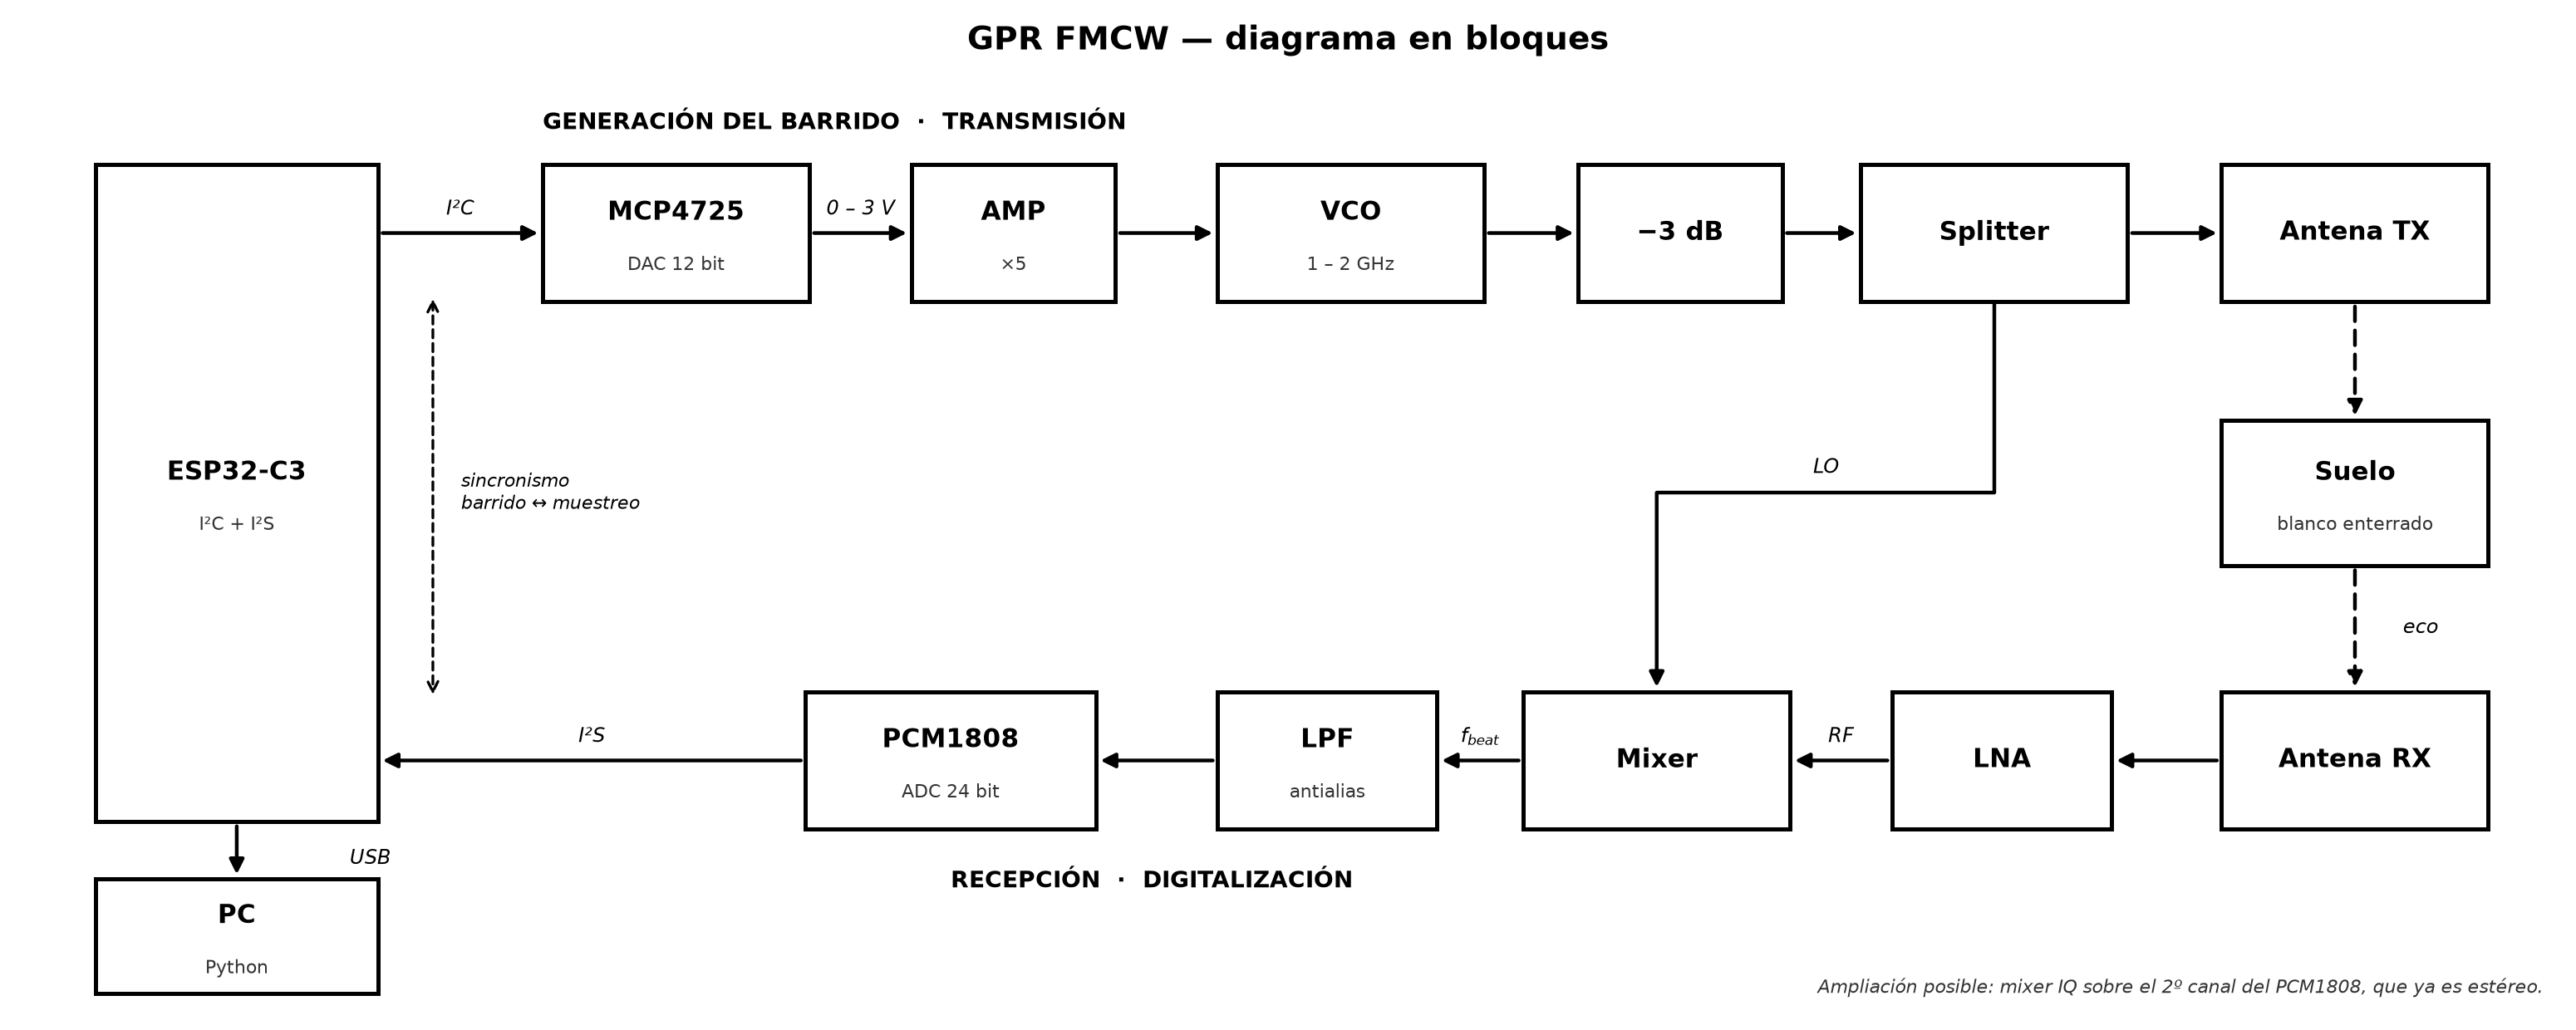
\includegraphics[width=\linewidth]{figuras/arquitectura/diagrama_bloques.png}
  \caption{Diagrama en bloques del GPR FMCW, versión de un solo canal
  (alcance de esta tesis). El PCM1808 es estéreo, así que el camino de
  hardware para un segundo canal en cuadratura (mezclador IQ) ya existe y
  queda como ampliación posible, sin implementar.}
  \label{fig:diagrama_bloques}
\end{figure}

\section{Principio de funcionamiento: FMCW sin efecto Doppler}
\label{sec:principio_fmcw_sin_doppler}

El GPR no se desplaza respecto del suelo durante una medición, por lo que,
a diferencia del radar automotriz, no hay efecto Doppler que desplace en
frecuencia la señal recibida. Como se estableció en la
Sección~\ref{sec:beat_freq}, esto tiene una consecuencia directa: las ramas
ascendente y descendente de la triangular producen la \textbf{misma}
frecuencia de batido, así que una sola rampa alcanza para estimar distancia
(no hace falta la asimetría subida/bajada que en radar automotriz se usa
para despejar velocidad).

La Figura~\ref{fig:principio_fmcw} ilustra este principio en tres paneles
alineados en el tiempo: (a) la frecuencia instantánea transmitida y recibida,
con el retardo $\tau$ y la frecuencia de batido $f_\text{beat}$ marcados;
(b) la diferencia de frecuencias entre ambas señales, mostrando que vale lo
mismo en el tramo de subida que en el de bajada; y (c) la tensión a la
salida del mezclador, que oscila a $f_\text{beat}$ salvo en los vértices de
la triangular, donde el retardo hace que $f_\text{tx}$ y $f_\text{rx}$
crucen y la diferencia caiga momentáneamente a cero.

\begin{figure}[H]
  \centering
  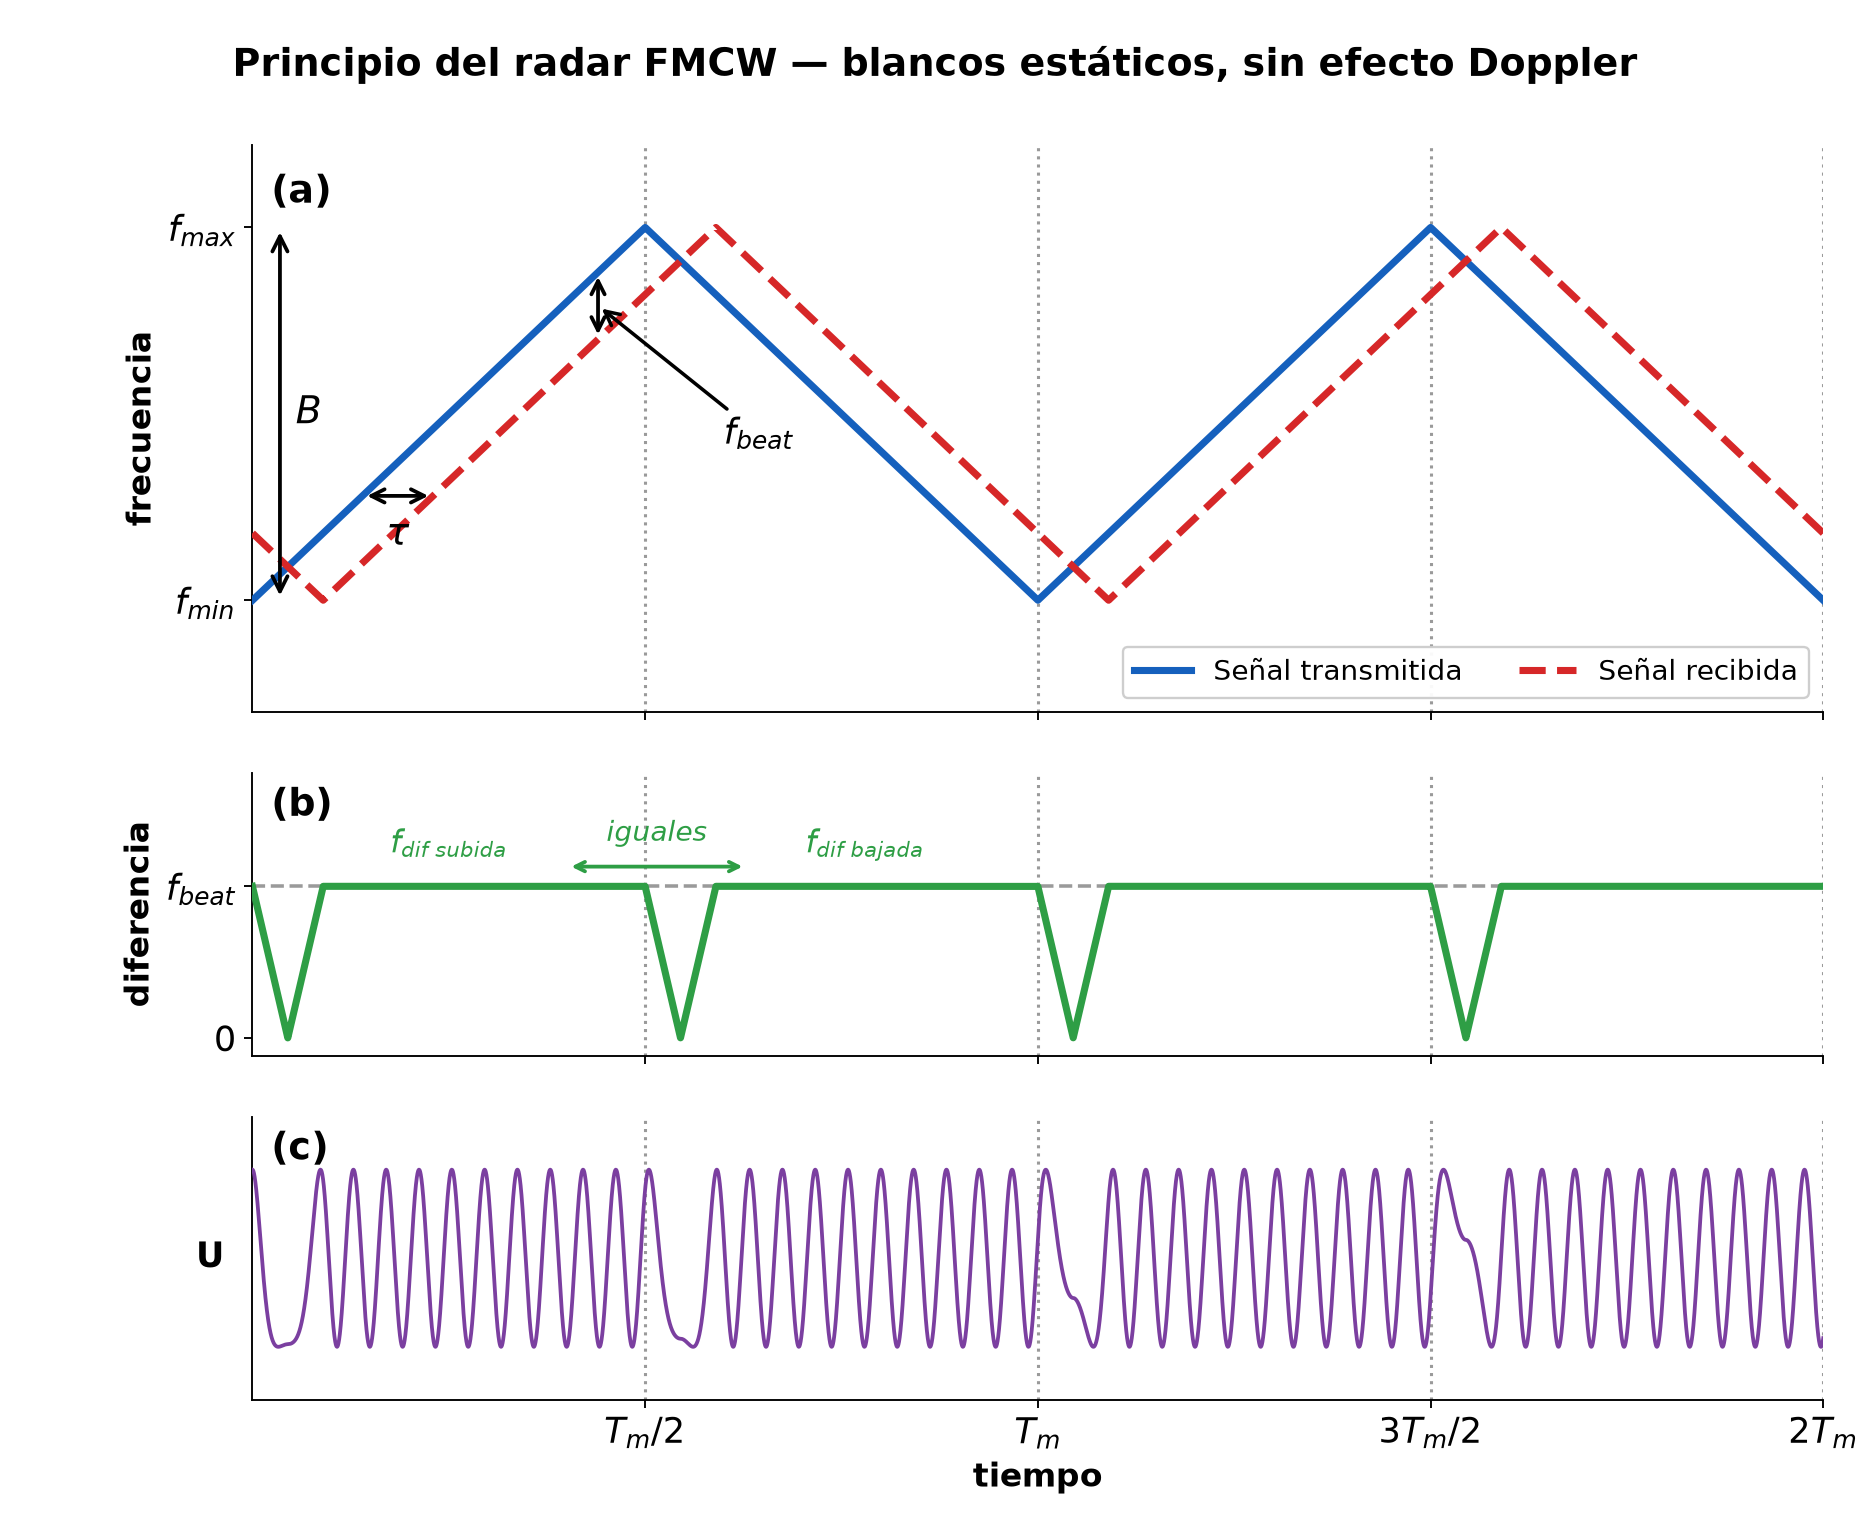
\includegraphics[width=0.85\linewidth]{figuras/arquitectura/principio_fmcw.png}
  \caption{Principio de funcionamiento del FMCW para un blanco estático, sin
  efecto Doppler (script \texttt{docs/principio\_fmcw.py}). Los valores de
  $\tau$, $T_m$ y $B$ usados en la figura son adimensionales y se eligieron
  para que el dibujo se lea bien, no para representar las magnitudes reales
  del sistema: en el radar real, $\tau/T_m$ es del orden de $10^{-7}$ para un
  blanco a $1\,\text{m}$, y a esa escala la señal recibida se superpondría
  visualmente por completo a la transmitida.}
  \label{fig:principio_fmcw}
\end{figure}

%============================================================
\chapter{Banco de Pruebas}
\label{ch:banco}
%============================================================

\section{Cadena de RF}
\label{sec:banco_rf}

La Figura~\ref{fig:banco_rf} muestra la primera versión armada de la
cadena de RF sobre una plaqueta de prueba, con los bloques rotulados a
mano: VCO, amplificador, atenuador, splitter y la etapa de mezcla hacia
la antena transmisora.

\begin{figure}[H]
  \centering
  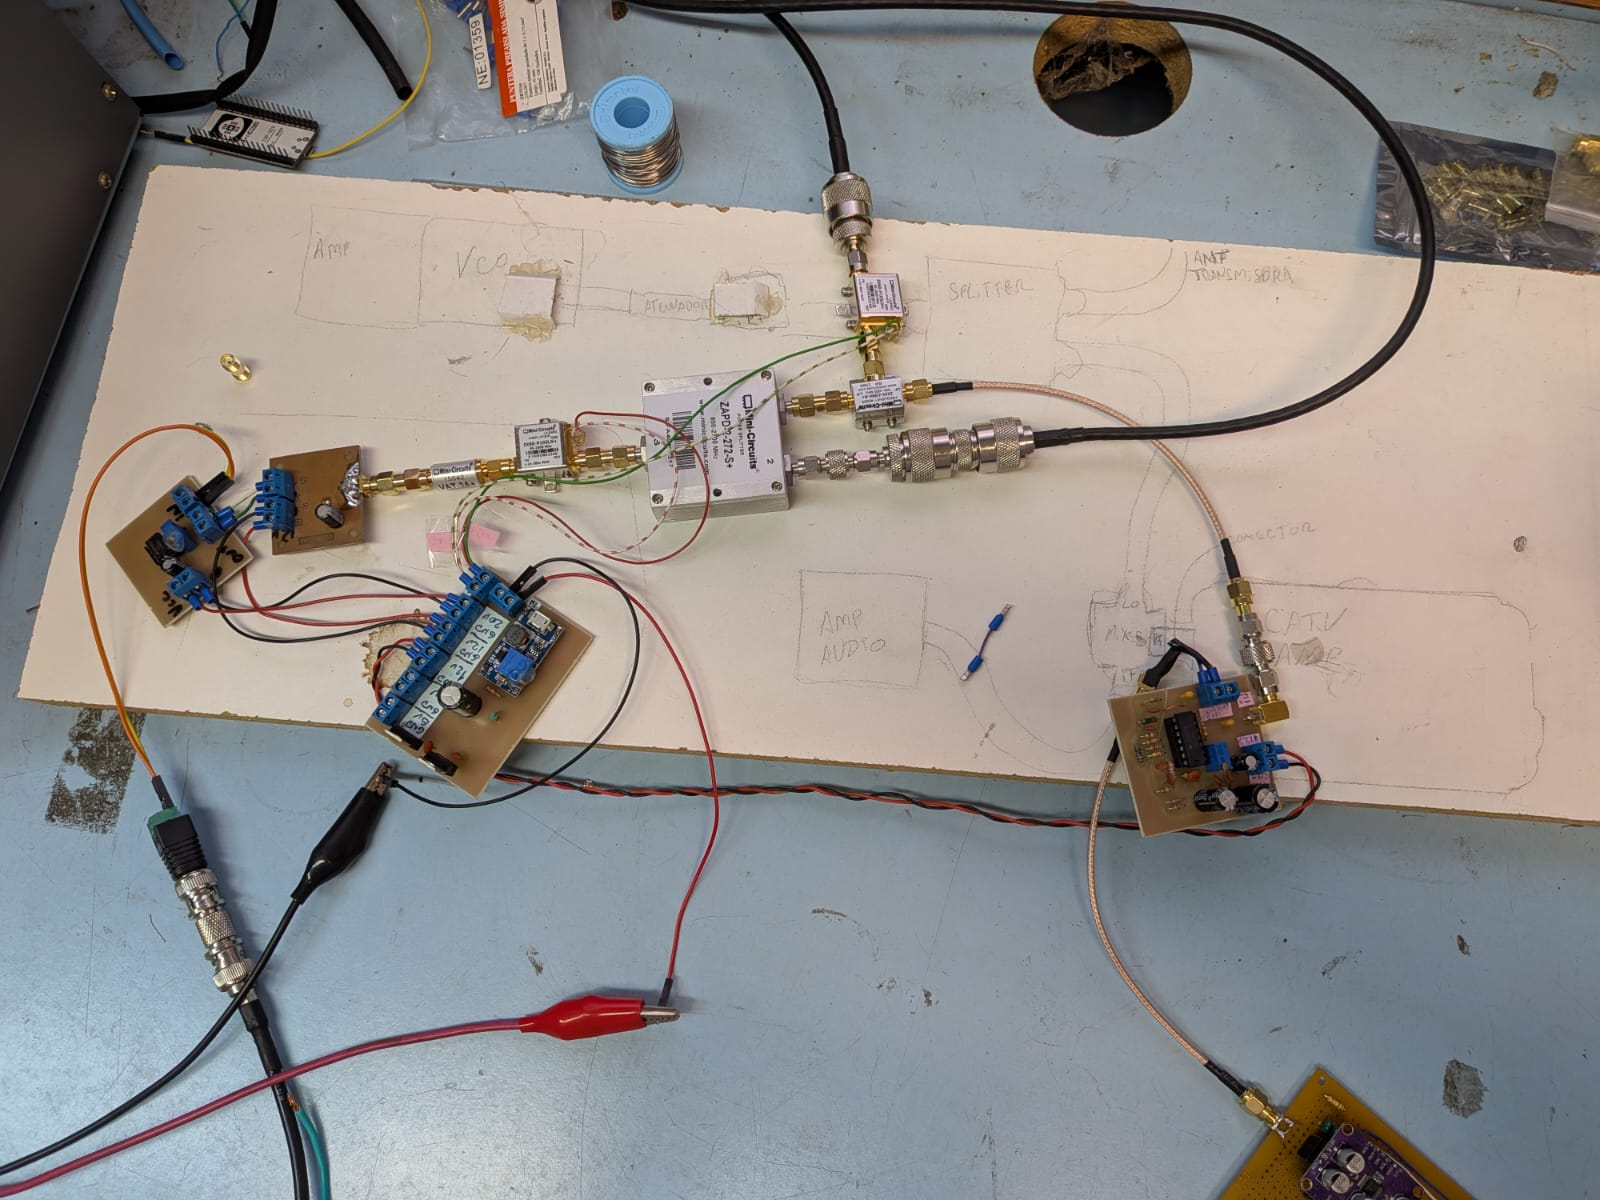
\includegraphics[width=0.85\linewidth]{figuras/banco/primer_banco_medicion1.jpeg}
  \caption{Primer banco de la cadena de RF: VCO, amplificador,
  atenuador y splitter interconectados sobre una plaqueta de prueba
  rotulada a mano.}
  \label{fig:banco_rf}
\end{figure}

\section{Banco de mediciones}
\label{sec:banco_completo}

Las Figuras~\ref{fig:banco_completo1} y~\ref{fig:banco_completo2}
muestran el banco completo de mediciones: fuente DC, generador de
funciones, la cadena de RF de la Figura~\ref{fig:banco_rf} y la
notebook corriendo el software de adquisición/análisis (el trazo verde
es la señal capturada y el azul su espectro).

\begin{figure}[H]
  \centering
  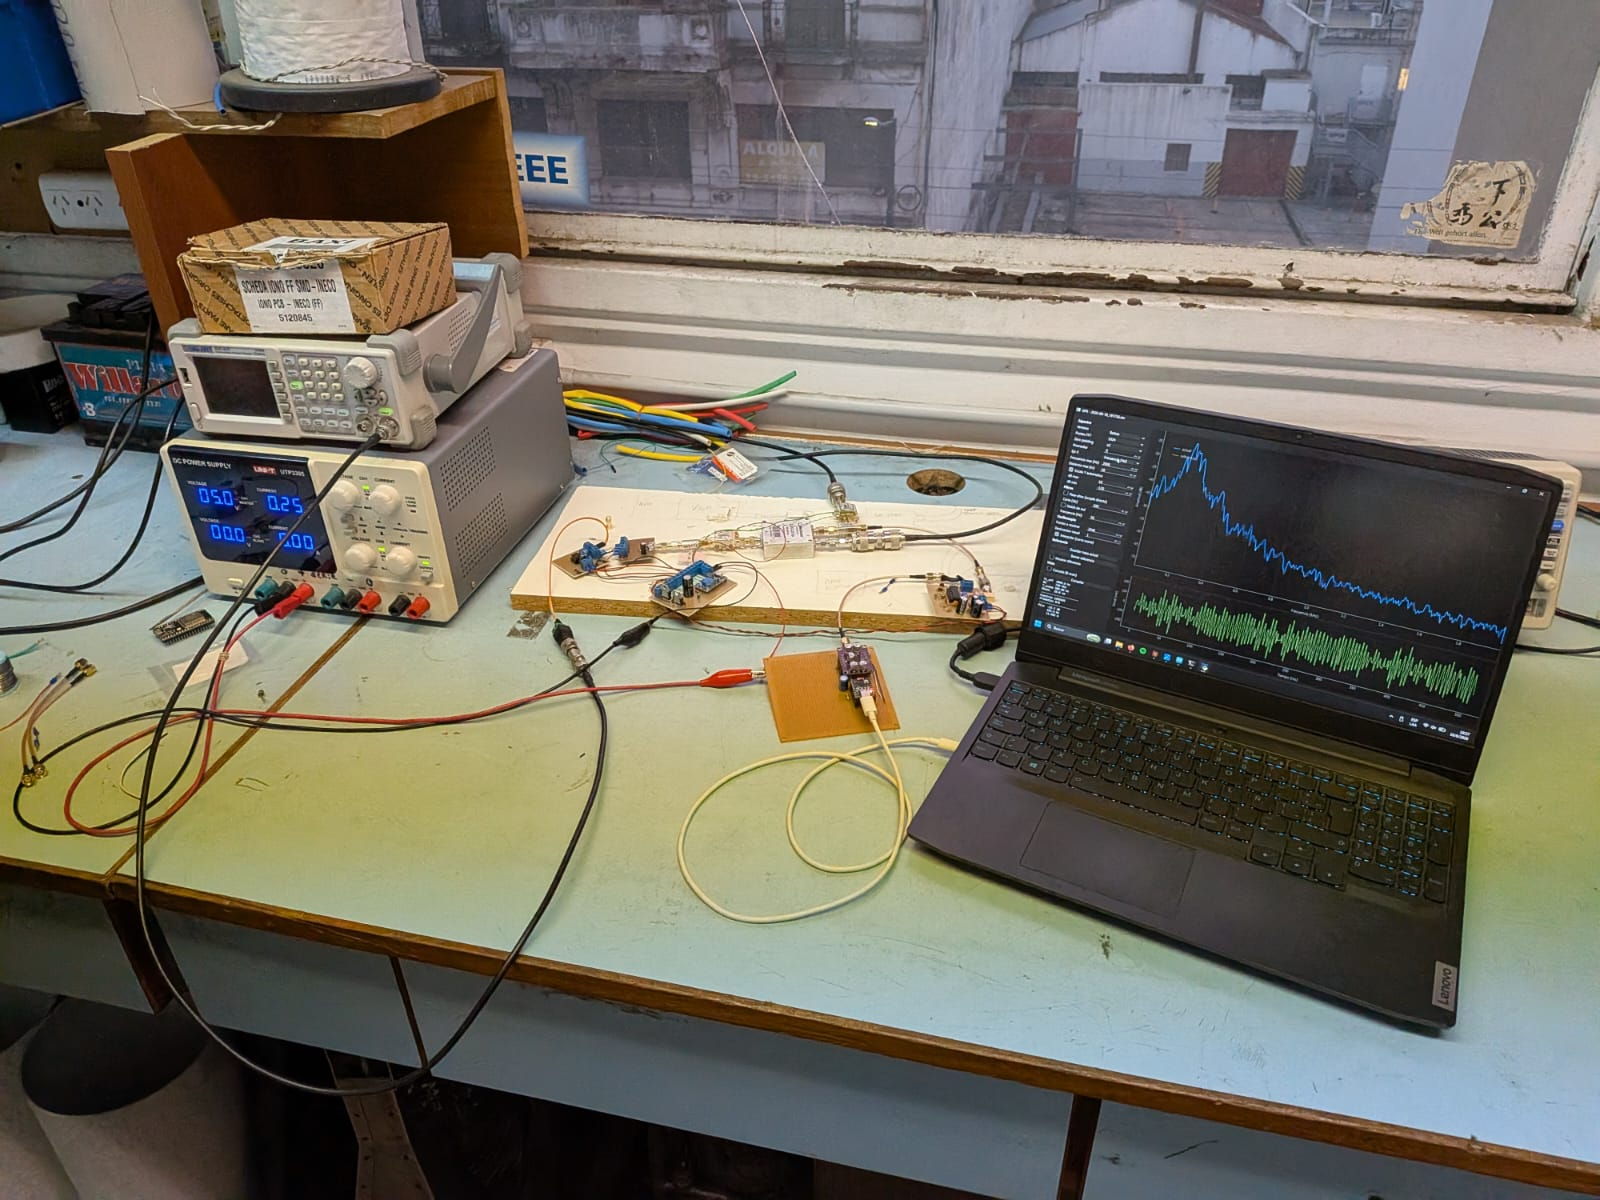
\includegraphics[width=0.95\linewidth]{figuras/banco/primer_banco_medicion2.jpeg}
  \caption{Banco de mediciones: fuente DC, generador de funciones,
  cadena de RF y notebook con el software de análisis.}
  \label{fig:banco_completo1}
\end{figure}

\begin{figure}[H]
  \centering
  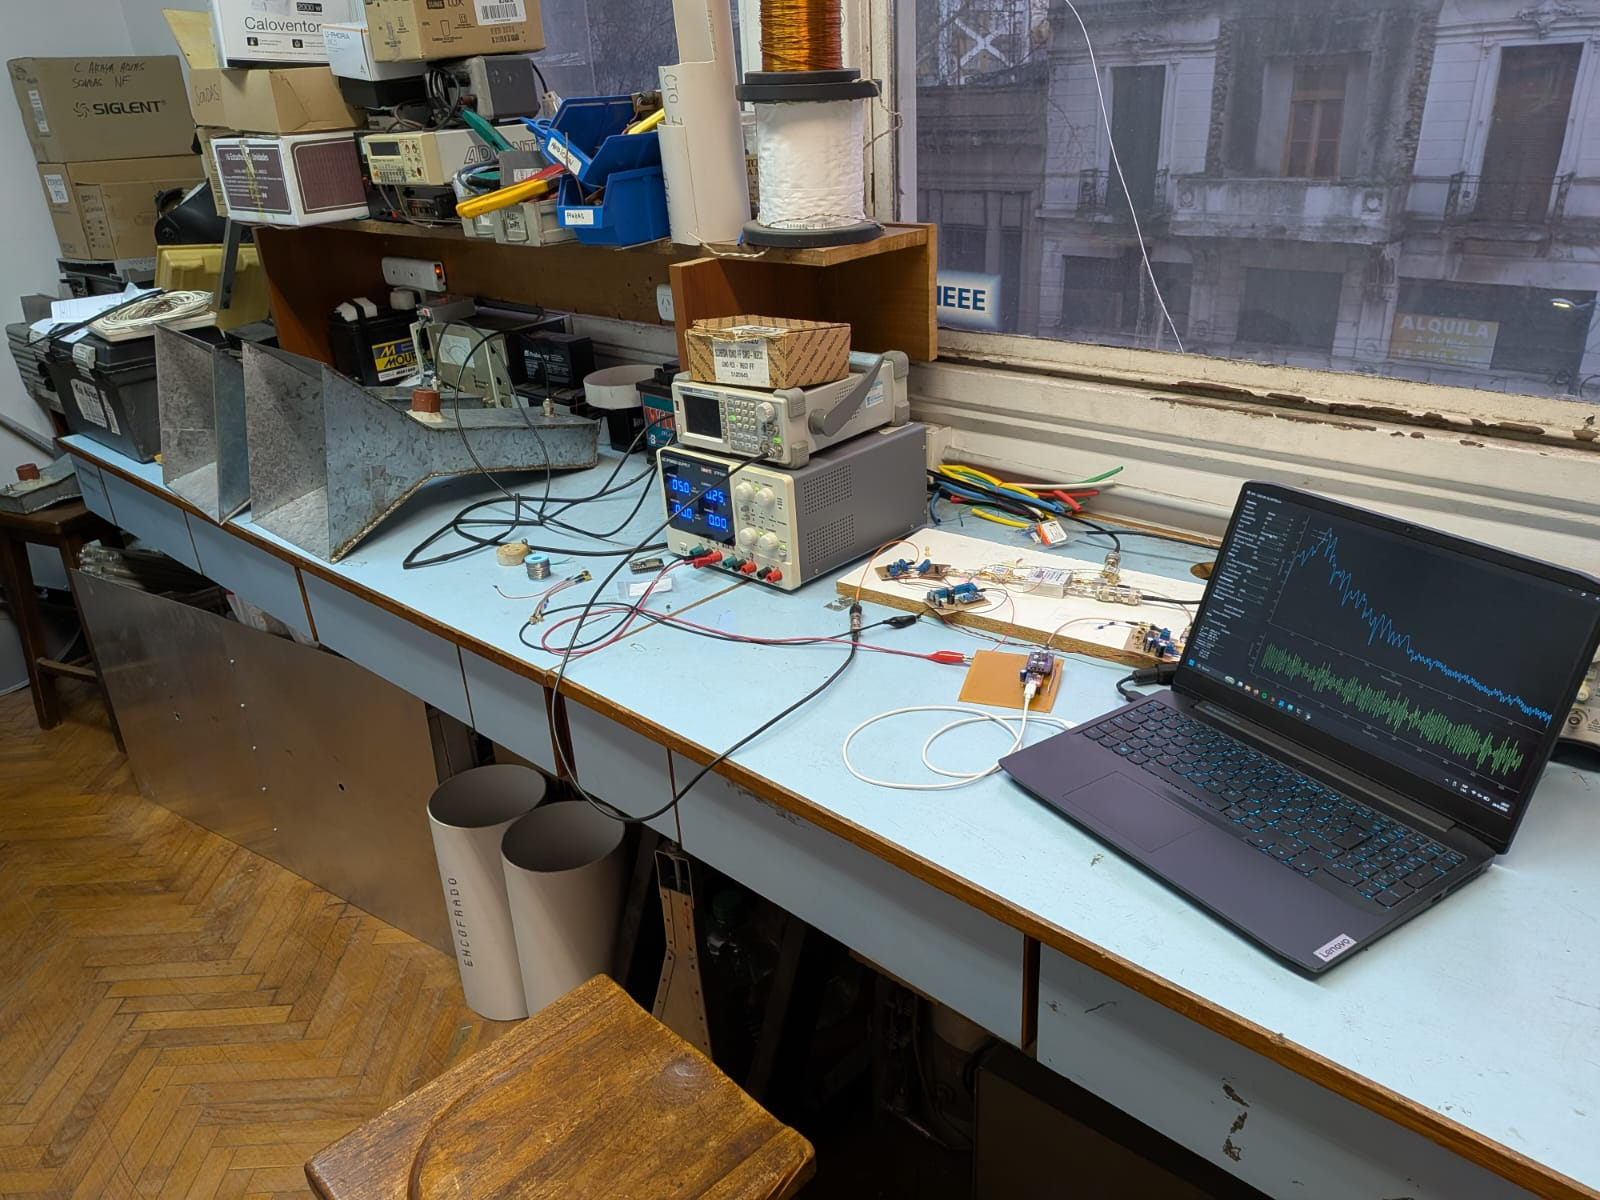
\includegraphics[width=0.95\linewidth]{figuras/banco/primer_banco_medicion3.jpeg}
  \caption{Banco de mediciones, vista general del puesto de trabajo.}
  \label{fig:banco_completo2}
\end{figure}

%============================================================
\chapter{Caracterización del VCO}
\label{ch:vco}
%============================================================

\section{Curva de sintonía del VCO}
\label{sec:curva_vco}

El VCO se caracterizó punto a punto, barriendo la tensión de control
$V_\text{in}$ de $0$ a $3{,}321\,\text{V}$ en pasos de $100\,\text{mV}$
(34 puntos) y midiendo la frecuencia de salida con un analizador de
espectro (precisión de $1\,\text{MHz}$). La Figura~\ref{fig:curva_vco}
muestra la curva resultante junto con la sensibilidad $dF/dV$.

\begin{figure}[H]
  \centering
  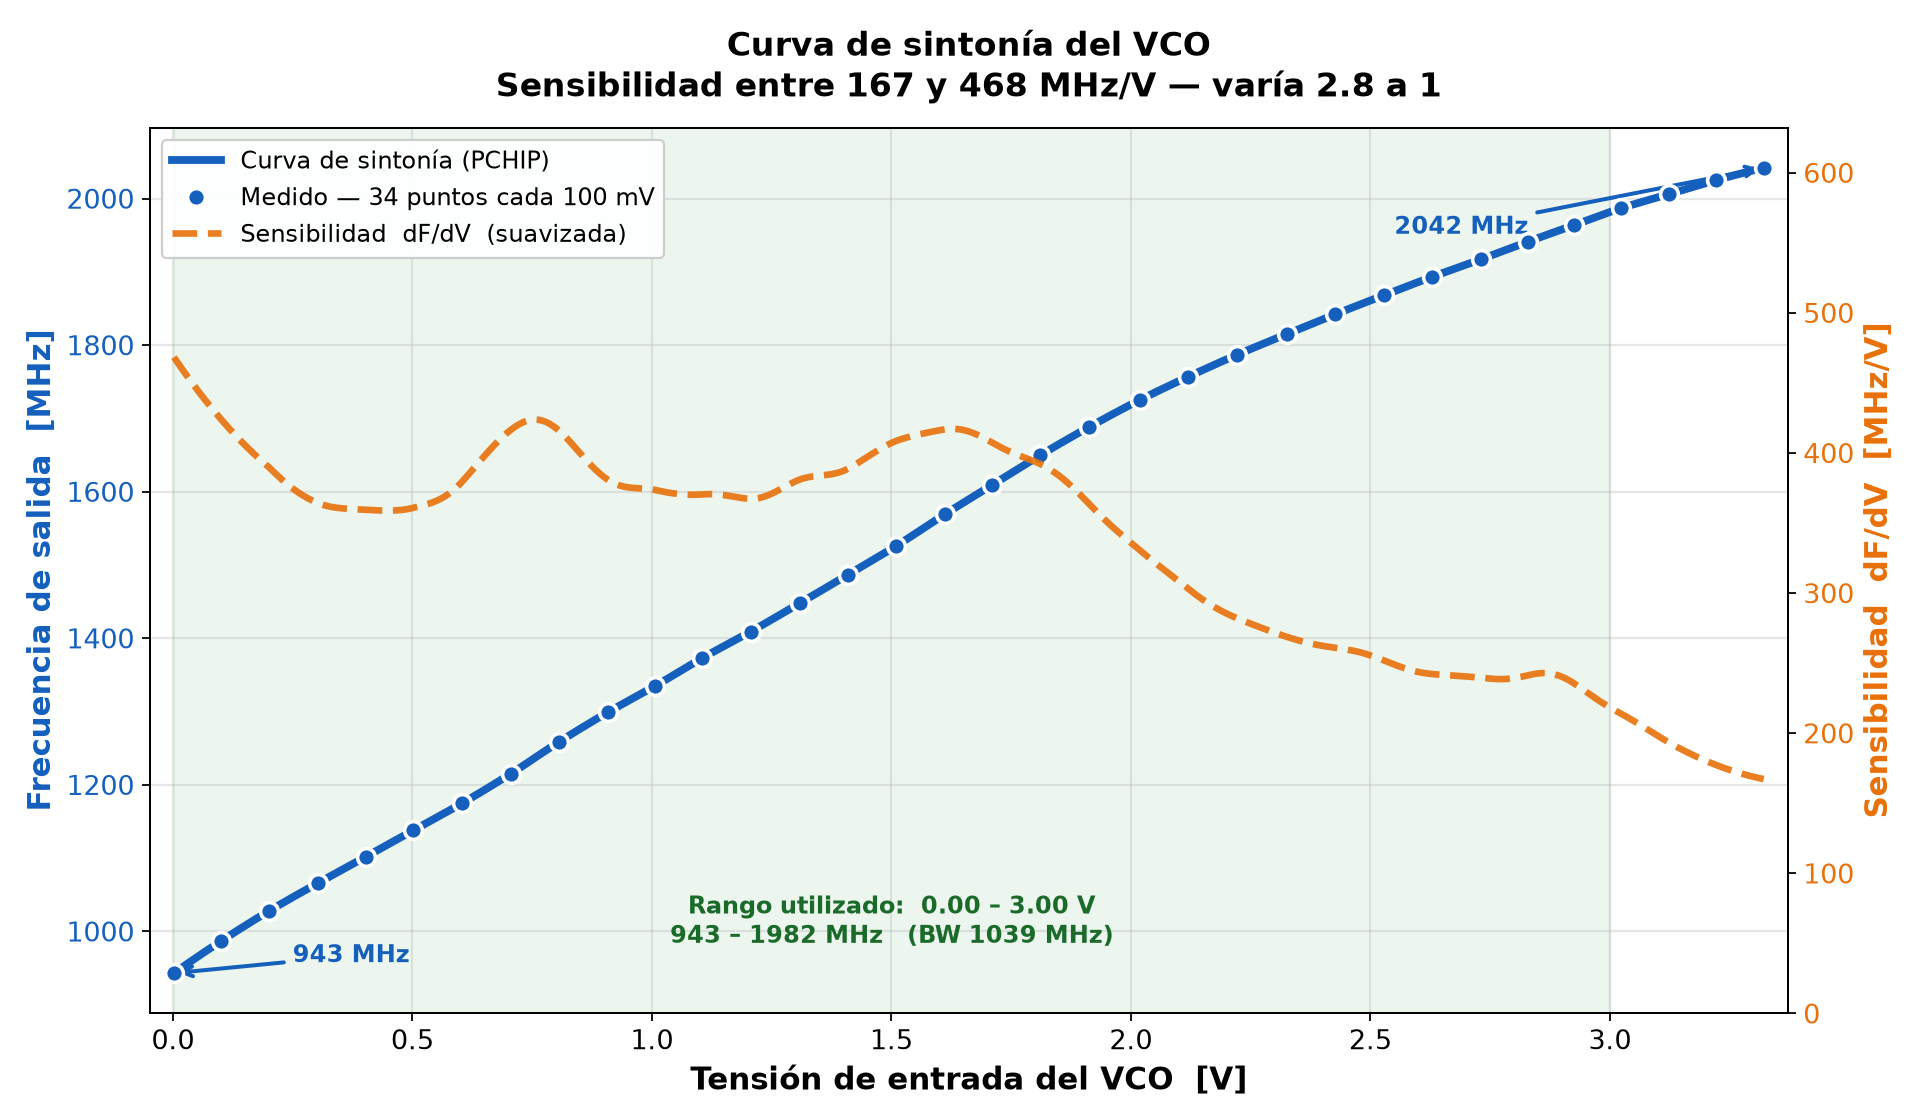
\includegraphics[width=0.95\linewidth]{figuras/vco/vco_frecuencia_vs_tension.png}
  \caption{Curva de sintonía medida del VCO: frecuencia de salida en
  función de la tensión de control $V_\text{in}$ (antes del mapeo a la
  tensión real de sintonía $V_\text{osc}$, más alta, que entrega el
  amplificador entre el DAC y el VCO). El rango sombreado indica los
  $0$--$3{,}00\,\text{V}$ que efectivamente se usan para generar la
  rampa del radar.}
  \label{fig:curva_vco}
\end{figure}

En el rango medido completo ($0{,}002$ a $3{,}321\,\text{V}$) la
frecuencia va de $943$ a $2042\,\text{MHz}$. La sensibilidad $dF/dV$
no es constante: varía entre $167$ y $468\,\text{MHz/V}$ (relación
$2{,}8$ a $1$ entre el extremo más y menos sensible), lo cual es la
razón por la que una rampa de tensión lineal no produce una rampa de
frecuencia lineal (se retoma la predistorsión en la
Sección~\ref{sec:rampa_dac}).

Para no exceder el rango seguro de operación del VCO ni del DAC, el
rango de tensión que efectivamente se usa para generar la rampa del
radar se acotó a $V_\text{in} \in [0{,}00,\ 3{,}00]\,\text{V}$, lo que
corresponde a una banda de $943$ a $1982\,\text{MHz}$
($BW = 1039\,\text{MHz}$).

\section{Tabla de valores medidos}
\label{sec:tabla_vco}

La Tabla~\ref{tab:vco_completa} lista los 34 puntos medidos.

\begin{longtable}{ccc@{\hspace{1.2cm}}ccc}
\caption{Caracterización medida del VCO: tensión de entrada $V_\text{in}$ (salida del DAC + amplificador, 34 puntos cada 100~mV), frecuencia de salida y, para los últimos 6 puntos, la tensión real tras el amplificador $V_\text{osc}$.}
\label{tab:vco_completa} \\
\toprule
$V_\text{in}$ [V] & $f$ [MHz] & $V_\text{osc}$ [V] & $V_\text{in}$ [V] & $f$ [MHz] & $V_\text{osc}$ [V] \\
\midrule
\endfirsthead
\toprule
$V_\text{in}$ [V] & $f$ [MHz] & $V_\text{osc}$ [V] & $V_\text{in}$ [V] & $f$ [MHz] & $V_\text{osc}$ [V] \\
\midrule
\endhead
\bottomrule
\endfoot
$0{,}002$ & 943 & --- & $1{,}710$ & 1609 & --- \\
$0{,}101$ & 987 & --- & $1{,}811$ & 1650 & --- \\
$0{,}201$ & 1028 & --- & $1{,}912$ & 1688 & --- \\
$0{,}303$ & 1066 & --- & $2{,}018$ & 1725 & --- \\
$0{,}403$ & 1102 & --- & $2{,}120$ & 1757 & --- \\
$0{,}502$ & 1138 & --- & $2{,}222$ & 1787 & --- \\
$0{,}604$ & 1175 & --- & $2{,}325$ & 1815 & --- \\
$0{,}705$ & 1215 & --- & $2{,}426$ & 1842 & --- \\
$0{,}807$ & 1259 & --- & $2{,}528$ & 1868 & --- \\
$0{,}908$ & 1299 & --- & $2{,}628$ & 1893 & --- \\
$1{,}007$ & 1335 & --- & $2{,}730$ & 1917 & --- \\
$1{,}105$ & 1373 & --- & $2{,}828$ & 1941 & $14{,}050$ \\
$1{,}206$ & 1409 & --- & $2{,}926$ & 1964 & $14{,}540$ \\
$1{,}309$ & 1448 & --- & $3{,}024$ & 1987 & $15{,}020$ \\
$1{,}410$ & 1487 & --- & $3{,}123$ & 2006 & $15{,}510$ \\
$1{,}510$ & 1526 & --- & $3{,}221$ & 2025 & $16{,}000$ \\
$1{,}611$ & 1569 & --- & $3{,}321$ & 2042 & $16{,}490$ \\
\end{longtable}


Para el último punto del barrido ($V_\text{in} = 3{,}321\,\text{V}$) se
midió una tensión de $16{,}490\,\text{V}$ a la entrada del VCO (tras el
amplificador entre el DAC y el VCO), que se encuentra dentro del rango
de funcionamiento del dispositivo (hasta $20\,\text{V}$).

\section{Predistorsión: linealización mediante interpolación PCHIP}
\label{sec:predistorsion_pchip}

Como se señaló en la Sección~\ref{sec:curva_vco}, la sensibilidad
$dF/dV$ del VCO no es constante. En un radar FMCW la frecuencia de
batido es proporcional a $dF/dt$, de modo que si la rampa de tensión
es lineal en el tiempo pero $dF/dV$ no lo es, la frecuencia tampoco
barre linealmente: el eco de un único blanco puntual queda repartido
sobre todo el rango de pendientes en lugar de concentrarse en una
única frecuencia de batido, y el pico de distancia se ensancha.

Para corregirlo se invierte la curva medida: en vez de recorrer la
tensión linealmente, se recorre la \emph{frecuencia} linealmente y se
calcula, para cada instante, qué tensión hace falta. La inversión se
hace ajustando la curva de 34 puntos (Tabla~\ref{tab:vco_completa})
con un interpolador PCHIP (\textit{Piecewise Cubic Hermite
Interpolating Polynomial}) tanto en el sentido $V\!\to\!F$ como en su
inversa $F\!\to\!V$; se eligió PCHIP en lugar de un spline cúbico
porque preserva la monotonía de los datos medidos sin generar
oscilaciones entre puntos que no están respaldadas por una medición.
La tabla resultante (1024 entradas, cuantizadas a los 12~bits del DAC
MCP4725) se calcula una única vez de forma offline con el script
\texttt{VCO/analisis\_vco.py} y se vuelca al firmware como
\texttt{tabla\_vco.h}, de modo que el ESP32-C3 solo indexa la tabla en
tiempo de ejecución sin necesidad de punto flotante.

La Figura~\ref{fig:curva_vco_completa} resume el procedimiento y su
resultado: arriba a la izquierda, la curva medida con el ajuste PCHIP
superpuesto y el rango efectivamente usado ($0$ a $3\,\text{V}$)
sombreado; arriba a la derecha, la sensibilidad punto a punto
$dF/dV$; abajo a la izquierda, la rampa de tensión que efectivamente
entrega el DAC con y sin predistorsión; abajo a la derecha, la
frecuencia resultante en función del tiempo, comparada con la recta
ideal.

\begin{figure}[H]
  \centering
  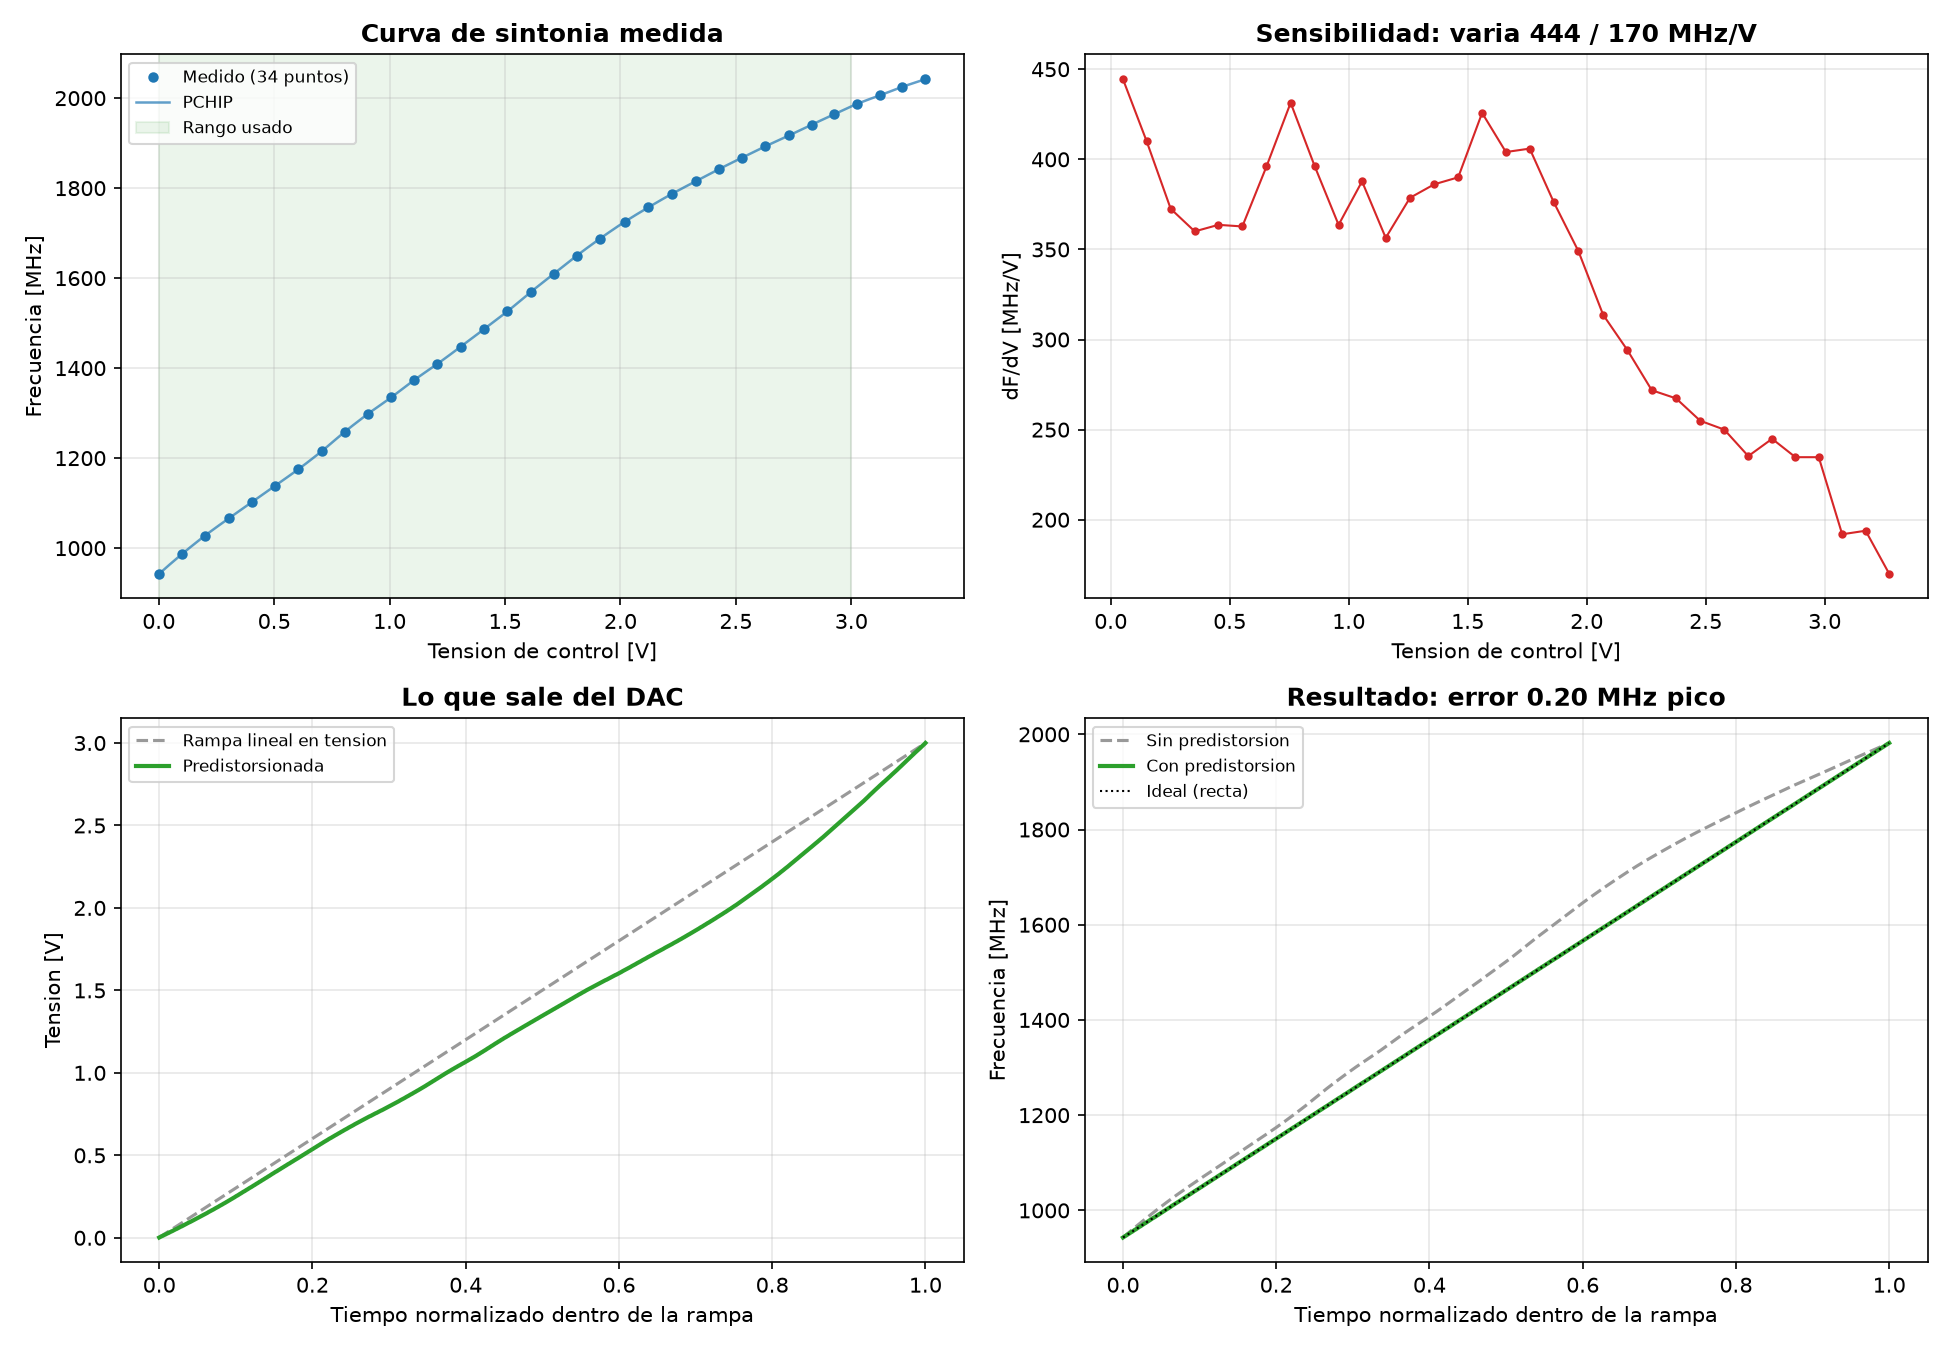
\includegraphics[width=0.95\linewidth]{figuras/vco/curva_vco.png}
  \caption{Linealización del barrido del VCO mediante predistorsión
  (script \texttt{VCO/analisis\_vco.py}). Arriba: curva de sintonía
  medida con ajuste PCHIP (izq.) y sensibilidad $dF/dV$ punto a punto
  sin suavizar (der.). Abajo: rampa de tensión del DAC con y sin
  predistorsión (izq.) y frecuencia resultante en función del tiempo
  normalizado, comparada con la recta ideal (der.).}
  \label{fig:curva_vco_completa}
\end{figure}

Sobre el rango útil $V_\text{in} \in [0{,}002,\ 3{,}000]\,\text{V}$
($943$ a $1982\,\text{MHz}$, $BW = 1039\,\text{MHz}$, consistente con
la Sección~\ref{sec:curva_vco}), \textbf{sin predistorsión} la
pendiente $dF/dt$ varía entre $0{,}68$ y $1{,}29$ veces su valor
medio: un blanco puntual a $1\,\text{m}$ se desparramaría, por este
efecto, entre aproximadamente $0{,}68$ y $1{,}29\,\text{m}$.
\textbf{Con predistorsión}, $dF/dt$ queda acotado entre $0{,}991$ y
$1{,}010$ veces el promedio (variación de apenas $\pm 1\%$), con un
error de frecuencia residual de $0{,}20\,\text{MHz}$ pico
($0{,}08\,\text{MHz}$ rms), equivalente al $0{,}020\%$ del ancho de
banda. El escalón de tensión del DAC de 12~bits
($3{,}300\,\text{V}/4095 \approx 0{,}806\,\text{mV}$) equivale
típicamente a $0{,}27\,\text{MHz}$, valor que fija el piso de
resolución de la tabla.

\textit{Nota sobre la sensibilidad graficada:} el panel superior
derecho de la Figura~\ref{fig:curva_vco_completa} usa la derivada
cruda punto a punto ($444$ a $170\,\text{MHz/V}$), distinta de la
sensibilidad ya reportada en la Sección~\ref{sec:curva_vco} ($167$ a
$468\,\text{MHz/V}$), que se calculó suavizando con un filtro
Savitzky--Golay sobre la curva PCHIP (script
\texttt{VCO/grafico\_vco.py}). La derivada cruda arrastra la
cuantización de la medición (frecuencia redondeada a $1\,\text{MHz}$,
pasos de $100\,\text{mV}$) y por eso exagera el rango de
sensibilidad; ambos cálculos coinciden en lo cualitativo (la
sensibilidad varía fuertemente y no es constante), pero difieren en
el valor puntual según el método de derivación utilizado.

\section{Rampa del DAC: señal triangular, con y sin predistorsión}
\label{sec:rampa_dac}

Se capturó con el osciloscopio la salida real del DAC MCP4725 (la
rampa de sintonía del VCO), con la predistorsión activada y
desactivada, y a dos frecuencias de repetición de la rampa (PRF) de
$50\,\text{ms}$ y $5\,\text{ms}$. La Figura~\ref{fig:capturas_dac}
muestra las cuatro capturas.

\begin{figure}[H]
  \centering
  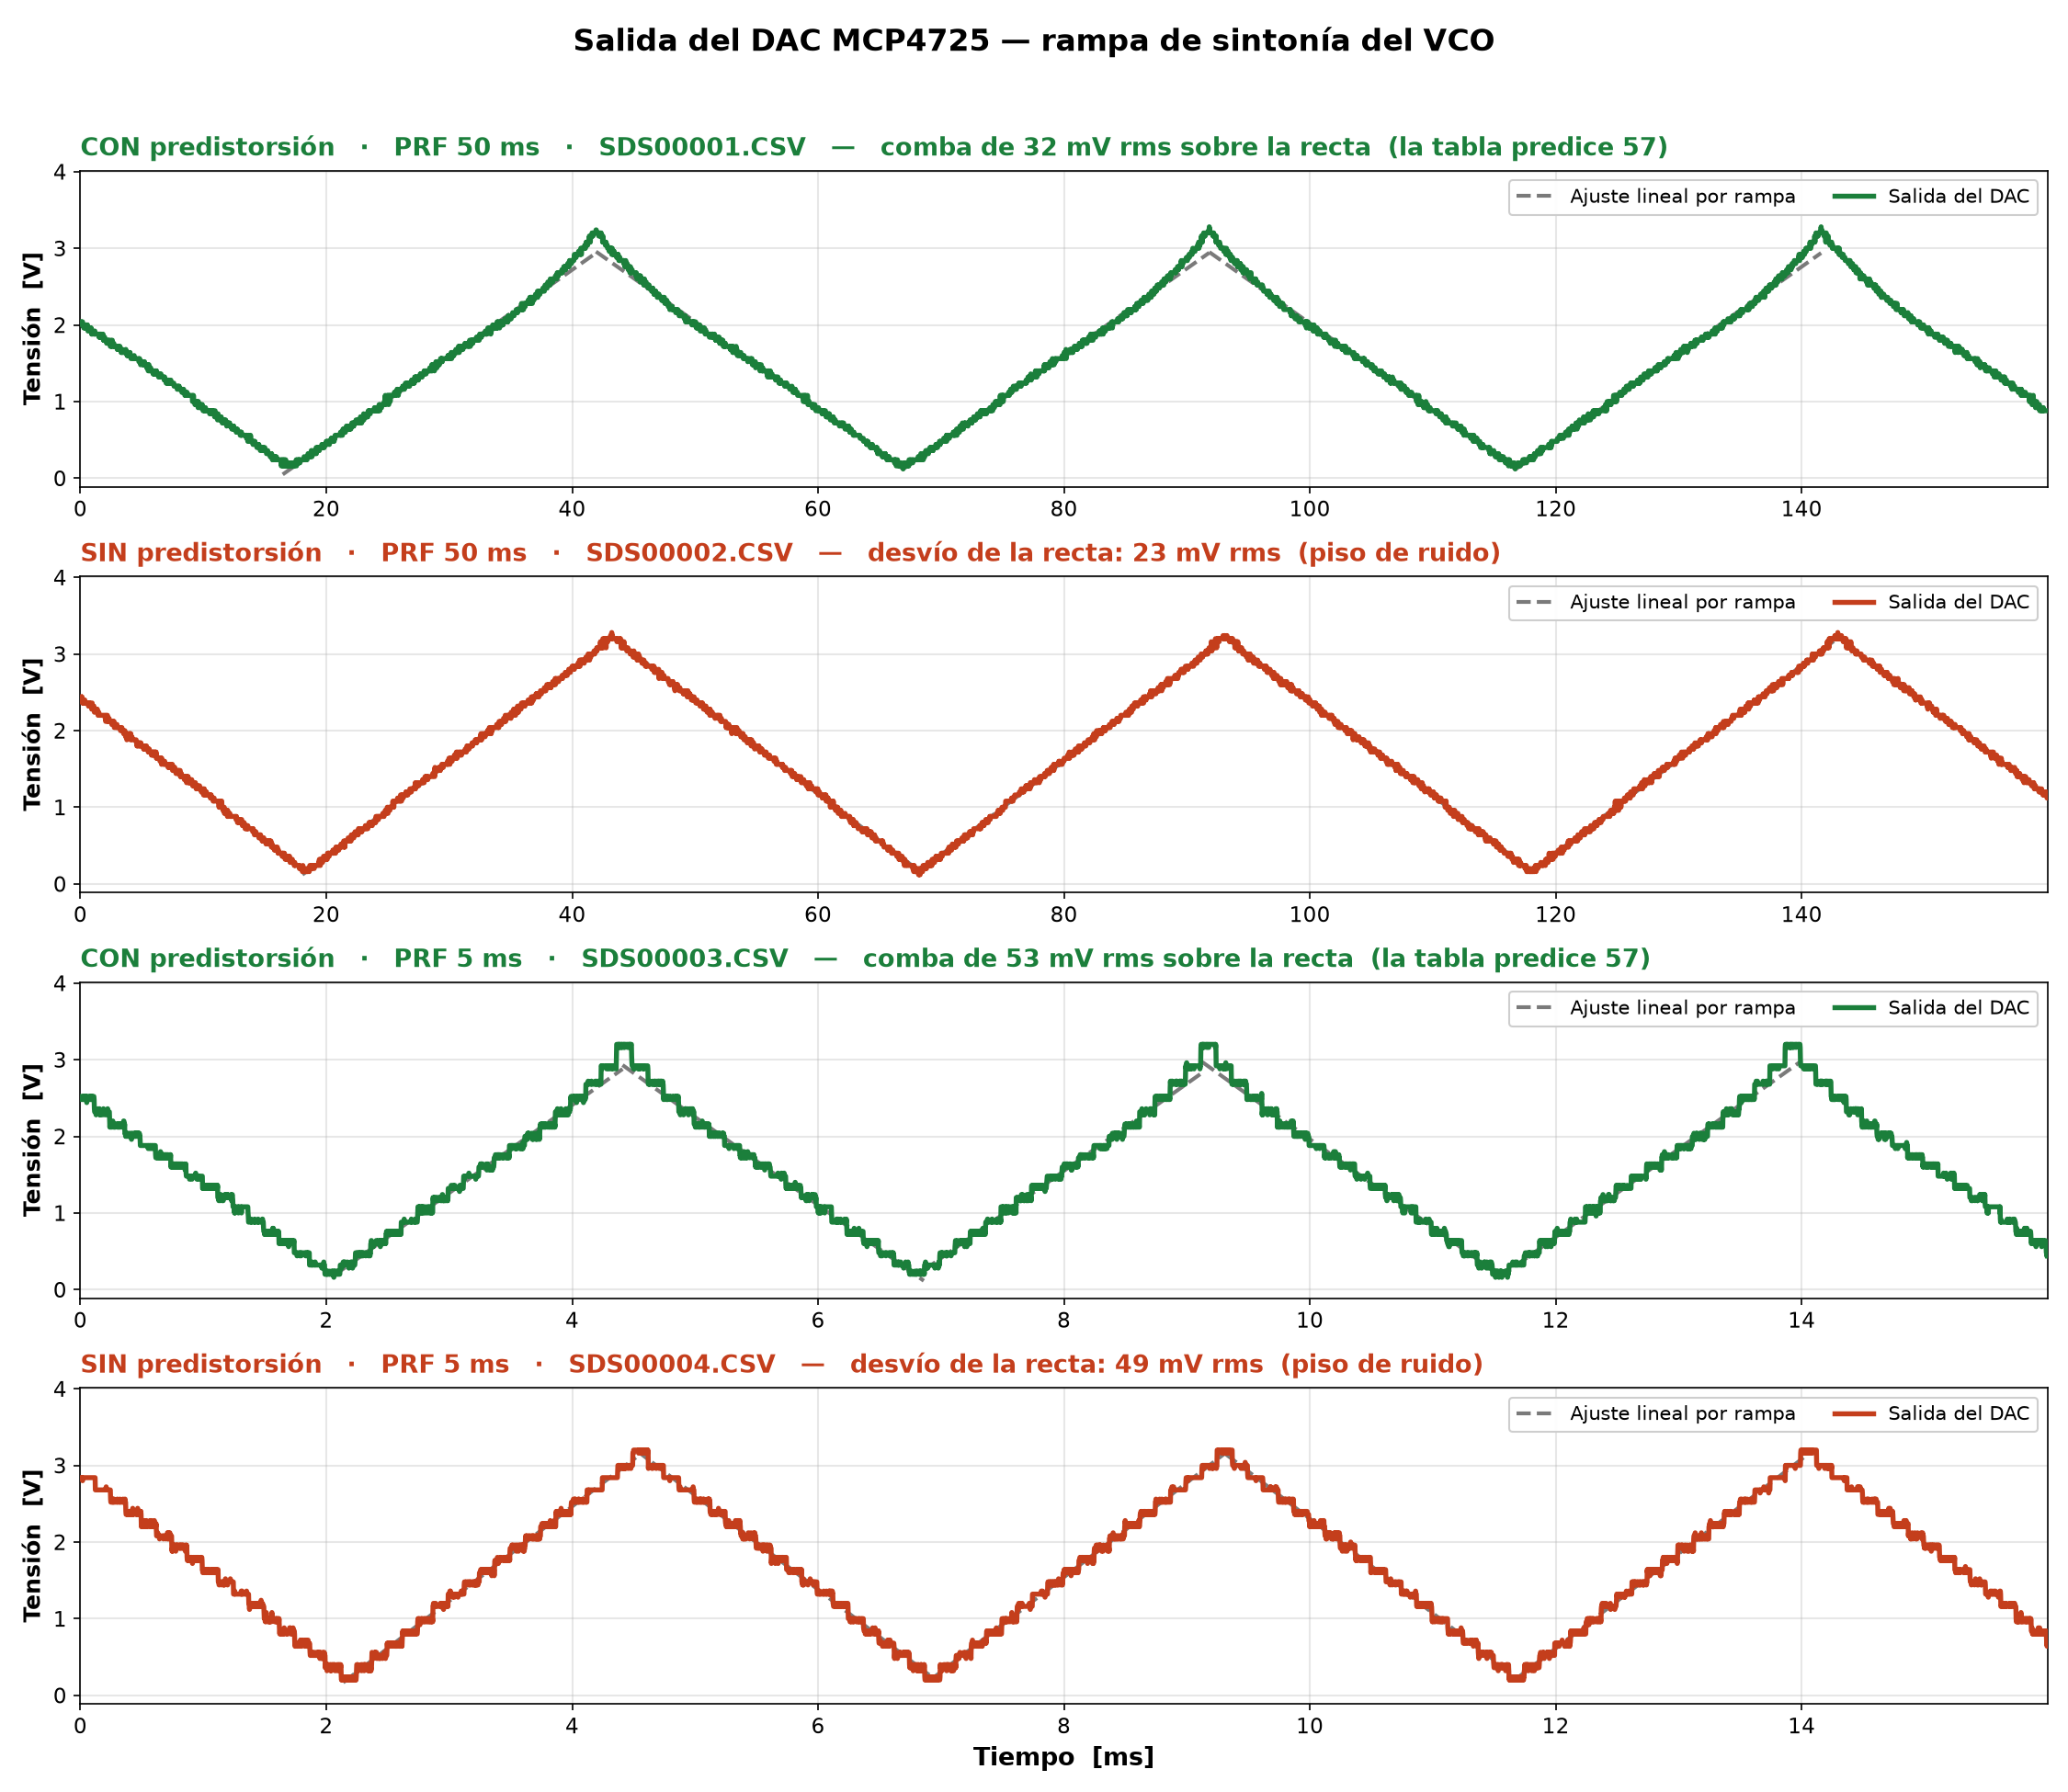
\includegraphics[width=0.95\linewidth]{figuras/vco/dac_capturas_osciloscopio.png}
  \caption{Salida del DAC MCP4725 (rampa de sintonía del VCO), con y sin
  predistorsión, a PRF de $50\,\text{ms}$ y $5\,\text{ms}$. Se indica el
  desvío RMS de cada rampa respecto de la recta ideal.}
  \label{fig:capturas_dac}
\end{figure}

Sin predistorsión, la rampa de tensión es lineal por construcción pero
—dado que $dF/dV$ no es constante— produce una rampa de frecuencia no
lineal. Con predistorsión, la tabla invertida (\texttt{tabla\_vco.h},
generada por \texttt{VCO/analisis\_vco.py}) corrige esto, y la comba
resultante sobre la rampa de tensión (los $32$--$53\,\text{mV}$~rms
medidos según la captura) es consistente con lo que predice la tabla
($57\,\text{mV}$~rms), dentro del ruido de cuantización del
osciloscopio.

%============================================================
\chapter{Filtro Pasabajos}
\label{ch:filtro}
%============================================================

\section{Objetivo y método de medición}
\label{sec:filtro_metodo}

Como ejercicio de práctica independiente del resto de la cadena de
RF, se caracterizó un filtro activo pasabajos con una etapa de
ganancia ajustable mediante potenciómetro, barriendo con un generador
de funciones senoidal y midiendo la tensión pico a pico de entrada y
de salida en dos posiciones del potenciómetro ($G=1$ y $G=2$) a lo
largo de un barrido logarítmico en frecuencia. La excitación de
entrada se mantuvo aproximadamente constante en
$3{,}113 \pm 0{,}045\,\text{V}_{pp}$ ($1{,}5\%$ de dispersión) a lo
largo de todo el barrido. Se registraron $52$ puntos para $G=2$ y
$24$ para $G=1$.

En cada punto el operador anotó el nivel de distorsión observado en
el osciloscopio (sin distorsión / poca distorsión / mucha distorsión
/ ruido), porque la tensión pico a pico de una onda distorsionada no
es la amplitud de su componente fundamental: un punto con distorsión
visible no representa la función transferencia lineal del filtro y
debe excluirse del ajuste cuantitativo. Con este criterio, los datos
se consideran válidos (sin distorsión) hasta $1750\,\text{Hz}$; por
encima de esa frecuencia (zona sombreada y trazo punteado en la
Figura~\ref{fig:respuesta_filtro}) las mediciones existen pero no
deben leerse como respuesta lineal del filtro.

\section{Respuesta en frecuencia}
\label{sec:filtro_respuesta}

La ganancia en banda de paso se calculó como la mediana de
$20\log_{10}(V_{pp,\text{out}}/V_{pp,\text{in}})$ sobre los puntos
válidos entre $200$ y $1750\,\text{Hz}$; las frecuencias de corte a
$-3\,\text{dB}$ se obtuvieron interpolando en escala logarítmica de
frecuencia el cruce con (ganancia de banda de paso $-3\,\text{dB}$).
Los resultados se resumen en la Tabla~\ref{tab:filtro_parametros} y
en la Figura~\ref{fig:respuesta_filtro}.

\begin{table}[H]
  \centering
  \caption{Parámetros medidos del filtro activo en las dos
  posiciones del potenciómetro de ganancia (banda de paso: mediana
  entre $200$ y $1750\,\text{Hz}$, puntos sin distorsión).}
  \label{tab:filtro_parametros}
  \begin{tabular}{lcc}
    \toprule
     & $G = 1$ & $G = 2$ \\
    \midrule
    Ganancia en banda de paso &
      $-0{,}17\,\text{dB}$ ($\times 0{,}981$) &
      $+6{,}51\,\text{dB}$ ($\times 2{,}115$) \\
    Corte inferior ($-3\,\text{dB}$) &
      $19{,}3\,\text{Hz}$ & $18{,}6\,\text{Hz}$ \\
    Corte superior ($-3\,\text{dB}$)\textsuperscript{*} &
      $20{,}3\,\text{kHz}$ & $17{,}5\,\text{kHz}$ \\
    \bottomrule
  \end{tabular}
\end{table}

\textsuperscript{*}Ambos valores de corte superior caen dentro de la
zona confirmada sin distorsión solo hasta $1750\,\text{Hz}$
(Sección~\ref{sec:filtro_metodo}); como se discute en la
Sección~\ref{sec:filtro_normalizada}, deben interpretarse como
\textbf{cota inferior} del ancho de banda real del filtro y no como
su valor exacto.

\begin{figure}[H]
  \centering
  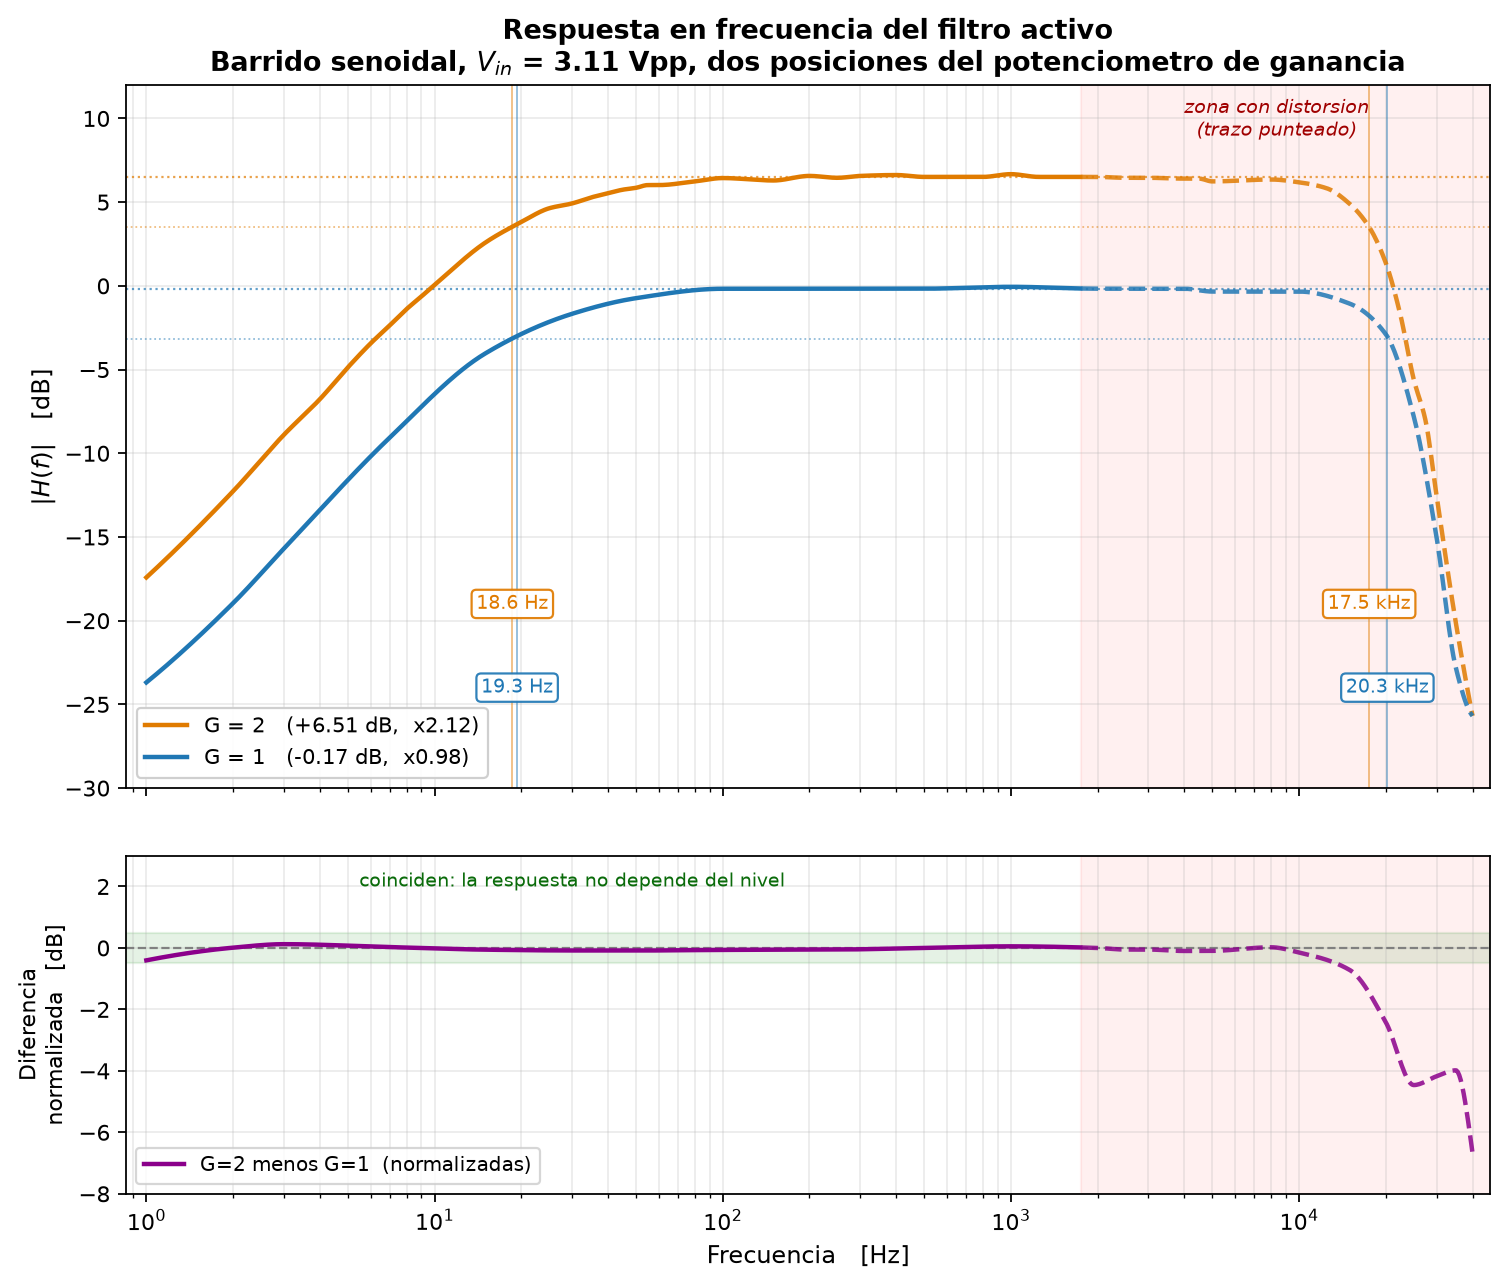
\includegraphics[width=0.95\linewidth]{figuras/filtro/respuesta_filtro.png}
  \caption{Respuesta en frecuencia del filtro activo, barrido
  senoidal con $V_{in} = 3{,}11\,\text{Vpp}$, en las dos posiciones
  del potenciómetro de ganancia. Arriba: respuesta absoluta, con las
  frecuencias de corte indicadas; el trazo se vuelve punteado a
  partir de la zona con distorsión. Abajo: diferencia entre ambas
  curvas normalizadas a su propia banda de paso.}
  \label{fig:respuesta_filtro}
\end{figure}

La ganancia adicional que aporta el potenciómetro entre las
posiciones $G=1$ y $G=2$ es de $6{,}68\,\text{dB}$ ($\times 2{,}157$).

\section{Comparación normalizada: separar el efecto de la ganancia
del efecto de la amplitud}
\label{sec:filtro_normalizada}

Si el filtro fuese lineal, normalizar cada curva a su propia banda de
paso debería hacer que ambas coincidan exactamente: el potenciómetro
escala la ganancia global pero no debería mover la posición de los
polos del filtro. El panel inferior de la
Figura~\ref{fig:respuesta_filtro} muestra que, en efecto, entre
$1\,\text{Hz}$ y $10\,\text{kHz}$ ambas curvas normalizadas coinciden
dentro de $0{,}40\,\text{dB}$.

Por encima de $15\,\text{kHz}$, sin embargo, divergen hasta
$6{,}68\,\text{dB}$ —exactamente la ganancia que aporta el
potenciómetro—. Esta divergencia ocurre precisamente en la zona ya
identificada como distorsionada (por encima de $1750\,\text{Hz}$,
Sección~\ref{sec:filtro_metodo}), donde la tensión pico a pico
medida deja de representar la amplitud de la componente fundamental.
La interpretación consistente con los datos es que ese flanco
superior depende del nivel de señal (la posición $G=2$, con más del
doble de amplitud de salida, entra antes en una zona no lineal del
circuito o de la medición) y no de la respuesta propia del filtro. En
consecuencia, el ancho de banda real del filtro es mayor que los
$\sim\!20\,\text{kHz}$ medidos en $G=1$, que a su vez ya es, por lo
dicho arriba, una cota inferior.

%============================================================
\chapter{Cables de RF: Retardo Eléctrico, Pérdidas y Calibración
  de Distancia}
\label{ch:cables}
%============================================================

En una prueba de banco con un blanco metálico a una distancia $d$
conocida (Sección~\ref{sec:prueba_metalica}), la frecuencia de batido
medida resultó sistemáticamente mayor que la predicha por la
ecuación~\eqref{eq:beat_freq_aire}: un blanco a $1\,\text{m}$ producía
una $f^*$ compatible con un blanco a varios metros. Este capítulo
muestra que el desvío no es un error del modelo de la
Sección~\ref{sec:beat_freq} sino un término que faltaba: \textbf{el
retardo eléctrico de los cables coaxiles} que conectan el splitter con
las antenas y con el oscilador local (LO) del mezclador. Se deduce ese
término a partir de la misma ecuación de propagación ya usada en la
Sección~\ref{sec:parametros_fmcw}
(ecuación~\eqref{eq:velocidad_medio}), se cuantifica su efecto sobre la
distancia estimada y el alcance no ambiguo, y se compara el juego de
cables original contra uno nuevo, más corto, caracterizando ambos con
un analizador de redes.

\section{El mezclador ve una diferencia de retardo, no una distancia}
\label{sec:cables_diferencia_retardo}

El mezclador de un radar FMCW homodino no tiene forma de saber cuánto
del retardo que ve entre sus dos entradas (RF y LO) proviene del
trayecto por el aire hacia el blanco y cuánto proviene del cableado que
llega hasta él. Ambos caminos comparten el mismo splitter de salida del
VCO, pero después divergen:

\begin{itemize}
  \item \textbf{Camino del LO} (corto): splitter $\to$ cable de
    longitud $L_\text{LO}$ $\to$ entrada LO del mezclador. En el banco
    de esta tesis ese tramo \emph{no es un cable}: el splitter y el
    mezclador van conectados directamente, con unos $5\,\text{cm}$ de
    unión, de modo que $L_\text{LO} \approx 0$
    (Sección~\ref{sub:cables_ejemplo}).
  \item \textbf{Camino de RF} (largo): splitter $\to$ cable de longitud
    $L_\text{TX}$ $\to$ antena transmisora $\to$ trayecto por el aire
    (ida y vuelta $2d$) $\to$ antena receptora $\to$ cable de longitud
    $L_\text{RX}$ $\to$ LNA $\to$ entrada RF del mezclador.
\end{itemize}

Se conserva $L_\text{LO}$ en la formulación aunque en este montaje
valga casi cero, porque es el término sobre el que se actúa si se
quiere cancelar el offset por diseño
(Sección~\ref{sec:cables_plantilla}).

La Figura~\ref{fig:cables_diagrama} esquematiza ambos caminos. El
retardo total que ve el mezclador es la suma del retardo eléctrico en
los cables más el retardo de propagación por el aire:

\begin{equation}
  \tau_\text{total} = \underbrace{\frac{L_\text{TX} + L_\text{RX}
  - L_\text{LO}}{v_p}}_{\displaystyle \tau_\text{cables}}
  \;+\; \underbrace{\frac{2d}{c}}_{\displaystyle \tau_\text{blanco}},
  \label{eq:tau_total}
\end{equation}

donde $v_p$ es la velocidad de propagación dentro del dieléctrico del
cable coaxil. Conviene definir el \textbf{desbalance neto de cableado}

\begin{equation}
  D \;=\; L_\text{TX} + L_\text{RX} - L_\text{LO},
  \label{eq:D_neto}
\end{equation}

que es la magnitud relevante: no importan las longitudes absolutas de
cada tramo, sino cuánto más largo es el camino de RF que el del LO. Si
$D = 0$ (cables perfectamente balanceados) el término de cables
desaparece y el mezclador mide únicamente $\tau_\text{blanco}$, que es
la situación que asume implícitamente la
ecuación~\eqref{eq:beat_freq_aire}.

\begin{figure}[H]
  \centering
  \begin{tikzpicture}[
      font=\small,
      box/.style={draw, rounded corners, minimum height=0.9cm,
        align=center, inner sep=4pt},
      arr/.style={-{Latex[length=2.2mm]}, thick},
      node distance=10mm and 8mm
    ]
    \node[box] (vco) {VCO};
    \node[box, right=of vco] (split) {Splitter};

    \node[box, above right=6mm and 18mm of split] (lo) {Mezclador\\(entrada LO)};
    \node[box, below right=6mm and 18mm of split] (tx) {Antena Tx};
    \node[box, right=32mm of tx] (rx) {Antena Rx};
    \node[box, above right=6mm and 8mm of rx] (lna) {LNA};
    \node[box, right=8mm of lo] (mix) {Mezclador};

    \draw[arr] (vco) -- (split);
    \draw[arr] (split.north east) -- node[above, sloped]{$L_\text{LO}$} (lo.west);
    \draw[arr] (split.south east) -- node[below, sloped]{$L_\text{TX}$} (tx.west);
    \draw[arr] (tx) -- node[above, font=\scriptsize]{aire, $2d$} (rx);
    \draw[arr] (rx) -- (lna);
    \draw[arr] (lna) -- node[above, sloped]{$L_\text{RX}$} (mix.south);
    \draw[arr] (lo) -- (mix);

    \node[align=center, below=2mm of mix, font=\scriptsize\itshape]
      {ve $\tau_\text{total} = \tau_\text{cables} + \tau_\text{blanco}$};
  \end{tikzpicture}
  \caption{Los dos caminos que llegan al mezclador. El del LO es corto
    y fijo ---en este banco, una conexión directa de $\approx
    5\,\text{cm}$---; el de RF incluye los cables a las antenas más el
    trayecto por el aire. El mezclador solo puede medir la diferencia
    de retardo entre ambos, no el retardo absoluto de ninguno.}
  \label{fig:cables_diagrama}
\end{figure}

\section{Velocidad de propagación en el cable: el factor de velocidad}
\label{sec:cables_vf}

La ecuación~\eqref{eq:velocidad_medio}, ya usada para la propagación en
el suelo, se aplica sin cambios al dieléctrico interno del cable
coaxil: $v_p = c/\sqrt{\varepsilon_{r,\text{cable}}}$. En cables de RF
esta razón se expresa habitualmente como el \textbf{factor de
velocidad} $\text{VF} = v_p/c = 1/\sqrt{\varepsilon_{r,\text{cable}}}$,
que el fabricante especifica en la hoja de datos. La
Tabla~\ref{tab:vf_cables} resume valores nominales típicos según el
dieléctrico.

\begin{table}[H]
  \centering
  \caption{Factor de velocidad nominal según el dieléctrico del cable
    coaxil (valores de catálogo típicos; a confirmar contra la hoja de
    datos del cable efectivamente utilizado).}
  \label{tab:vf_cables}
  \begin{tabular}{lcc}
    \toprule
    \textbf{Dieléctrico} & \textbf{Cables típicos} & \textbf{VF} \\
    \midrule
    Polietileno sólido      & RG-58, RG-213 & $\approx 0{,}66$ \\
    PTFE (teflón) sólido    & Semirrígido   & $\approx 0{,}70$ \\
    Polietileno espumado    & RG-8X espuma  & $\approx 0{,}78$ \\
    \bottomrule
  \end{tabular}
\end{table}

\textbf{El cable es más lento que el aire.} Con $\text{VF} = 0{,}66$,
un metro de cable tarda lo mismo que $1/0{,}66 \approx 1{,}52\,\text{m}$
de aire: es la razón por la que el retardo de los cables pesa más de
lo que la intuición geométrica sugiere.

\section{Retardo neto y distancia aparente}
\label{sec:cables_offset}

Identificando en la ecuación~\eqref{eq:tau_total} el término de cables
y sustituyéndolo en la ecuación~\eqref{eq:beat_freq} (usando
$S = 2B/T_c$, Sección~\ref{sec:parametros_fmcw}), la frecuencia de
batido medida es

\begin{equation}
  f^*_\text{medido} = S\,\tau_\text{total}
  = \underbrace{\frac{4Bd}{c\,T_c}}_{f^*(d),\ \text{ec.}~\eqref{eq:beat_freq_aire}}
  \;+\; \underbrace{\frac{2B}{T_c}\cdot\frac{D}{\text{VF}\cdot c}}_{f_\text{offset}}.
  \label{eq:f_offset}
\end{equation}

Aplicando la inversión de la ecuación~\eqref{eq:d_estimada} a
$f^*_\text{medido}$, el offset en frecuencia se traduce en un offset
constante en la distancia estimada, \textbf{independiente de $T_c$ y
de $d$}:

\begin{equation}
  \boxed{
    \hat{d} = d + d_\text{offset},
    \qquad
    d_\text{offset} = \frac{D}{2\,\text{VF}}.
  }
  \label{eq:d_offset}
\end{equation}

Es un corrimiento aditivo, no un factor de escala: la pendiente de
$\hat d$ respecto de $d$ sigue siendo $1$. Esto explica una observación
del banco que a primera vista resulta contraintuitiva: al acercar o
alejar el blanco, la frecuencia de batido bajaba o subía exactamente
como predice la ecuación~\eqref{eq:beat_freq_aire} —el sistema
\emph{medía bien}— pero el valor absoluto de $\hat d$ estaba corrido
por una constante ajena al blanco.

\subsection{Ejemplo numérico}
\label{sub:cables_ejemplo}

Con los cables originales del banco ---dos RG-58 desparejos,
$L_\text{TX} = 3\,\text{m}$ y $L_\text{RX} = 2{,}6\,\text{m}$--- y
$\text{VF} = 0{,}66$ (polietileno sólido, Tabla~\ref{tab:vf_cables}).

\textbf{En este montaje el camino del LO no lleva cable}: el splitter y
el mezclador van conectados directamente, con unos $5\,\text{cm}$ de
unión. Ese tramo aporta $0{,}25\,\text{ns}$, es decir $3{,}8\,\text{cm}$
de distancia aparente ---bastante menos que la resolución de
$14{,}4\,\text{cm}$ del radar---, así que $L_\text{LO}$ es despreciable
y $D \approx L_\text{TX} + L_\text{RX} = 5{,}55\,\text{m}$:

\begin{equation*}
  d_\text{offset} = \frac{5{,}55}{2 \times 0{,}66} \approx 4{,}20\,\text{m}.
\end{equation*}

Que $L_\text{LO}$ sea despreciable es una \emph{mala} noticia, no una
simplificación afortunada: es el único término de la
ecuación~\eqref{eq:D_neto} que resta, y no está restando nada. Todo el
cable de antena se paga entero.

Nótese además que esa ecuación solo pide la \emph{suma} $L_\text{TX} +
L_\text{RX}$: que los dos cables de antena sean de distinto largo no
agrega ningún término. El desbalance que importa es el que hay entre el
camino de RF y el del LO, no el que hay entre TX y RX.

Este offset es constante en distancia pero, al pasar por
$f_\text{offset} = S\,D/(\text{VF}\,c)$, depende de $T_c$ porque $S$
depende de $T_c$. La Tabla~\ref{tab:cables_ejemplo} evalúa
$f_\text{offset}$ y la $f^*_\text{medido}$ total esperada para un
blanco a $d = 1\,\text{m}$, con $B = 1\,\text{GHz}$.

\begin{table}[H]
  \centering
  \caption{Frecuencia de batido esperada para un blanco a
    $d = 1\,\text{m}$, con y sin el aporte de los cables originales
    ($D = 5{,}55\,\text{m}$, $\text{VF} = 0{,}66$). $d_\text{offset}
    = 4{,}20\,\text{m}$ es constante; lo que cambia con $T_c$ es a
    cuántos Hz equivale.}
  \label{tab:cables_ejemplo}
  \begin{tabular}{cccc}
    \toprule
    $T_c$ & $f^*(d=1\,\text{m})$ & $f_\text{offset}$
      & $f^*_\text{medido}$ \\
    \midrule
    $40\,\text{ms}$  &  $334\,\text{Hz}$ & $1402\,\text{Hz}$ & $1736\,\text{Hz}$ \\
    $80\,\text{ms}$  &  $167\,\text{Hz}$ &  $701\,\text{Hz}$ &  $868\,\text{Hz}$ \\
    $160\,\text{ms}$ &   $83\,\text{Hz}$ &  $351\,\text{Hz}$ &  $434\,\text{Hz}$ \\
    \bottomrule
  \end{tabular}
\end{table}

La fila de $T_c = 80\,\text{ms}$ es la que se comparó contra el banco:
el modelo predice $868\,\text{Hz}$ para un blanco a $1\,\text{m}$, y lo
observado en la medición superaba los $800\,\text{Hz}$. El acuerdo no
debe leerse como más fino de lo que es ---el $\text{VF}$ real sigue
siendo un valor de catálogo, no medido--- pero deja el orden de
magnitud fuera de discusión: el aporte de los cables es varias veces el
del blanco.

\section{Corrección: calibración con un punto de distancia conocida}
\label{sec:cables_calibracion}

Como $d_\text{offset}$ es un corrido de origen y no una escala, alcanza
con \textbf{un único} punto de calibración: colocar un blanco a una
distancia $d_\text{real}$ conocida, medir la $\hat d$ cruda que entrega
el sistema, y restar:

\begin{equation}
  d_\text{offset}^\text{medido} = \hat d - d_\text{real}.
  \label{eq:offset_medido}
\end{equation}

Con dos o más puntos a distancias distintas puede además ajustarse por
cuadrados mínimos una recta $\hat d = a\,d_\text{real} + b$, lo que
sirve como \textbf{verificación}: si el modelo de este capítulo es
correcto, $a$ debe dar $\approx 1$ y $b$ debe coincidir con el
$d_\text{offset}$ predicho por la
ecuación~\eqref{eq:d_offset} a partir de las longitudes de cable
medidas físicamente. Un valor de $a$ alejado de $1$ señala que el
problema no está en los cables sino en otro parámetro del sistema (por
ejemplo, un $T_c$ mal configurado respecto del que efectivamente
entrega el generador).

\section{Pérdidas de inserción: lo que los cables cuestan aparte del retardo}
\label{sec:cables_perdidas}

El retardo de los cables puede anularse por diseño, agregándole al
camino del LO tanto cable como suman $L_\text{TX} + L_\text{RX}$ para
que $D = 0$ en la ecuación~\eqref{eq:D_neto}. La \textbf{atenuación} de
los cables, en cambio, no se cancela nunca: cada tramo atenúa la señal
que lo atraviesa sin importar cuánto midan los otros ---y esa maniobra,
de hecho, \emph{agrega} atenuación en el LO en vez de quitarla. Un
coaxil atenúa más cuanto:

\begin{itemize}
  \item más alta es la frecuencia (la pérdida por efecto pelicular en
    el conductor crece aproximadamente con $\sqrt{f}$, y la pérdida en
    el dieléctrico crece aproximadamente en forma lineal con $f$);
  \item más largo es el tramo (la atenuación en dB es proporcional a la
    longitud);
  \item menor es el diámetro del conductor central y peor el
    dieléctrico (por eso el RG-213, con un conductor más grueso que el
    RG-58, atenúa menos por metro a igual frecuencia).
\end{itemize}

Esta pérdida golpea al sistema en dos lugares distintos de la cadena
de la Figura~\ref{fig:cables_diagrama}: la atenuación de
$L_\text{TX}$ resta potencia efectivamente radiada, y la de
$L_\text{RX}$ resta señal a la entrada del LNA \emph{antes} de que se
amplifique, empeorando directamente la figura de ruido de toda la
cadena. Acortar los cables reduce el retardo (Sección~\ref{sec:cables_offset})
\textbf{y} la atenuación al mismo tiempo: a diferencia de la elección
de $T_c$ (Capítulo~\ref{ch:senal_if}), acá no hay dos efectos en
sentidos opuestos que haya que balancear. El valor exacto de
atenuación en la banda de $943$ a $1982\,\text{MHz}$ depende del cable
concreto y se mide, no se supone: queda planteado como parte de la
caracterización de la Sección~\ref{sec:cables_plantilla}.

\section{Caracterización propuesta: cables originales vs. cables nuevos}
\label{sec:cables_plantilla}

Se armó un segundo juego de dos cables de $1\,\text{m}$ en RG-213 para
reemplazar los originales (RG-58 de $3\,\text{m}$ y $2{,}6\,\text{m}$).

\textbf{Por qué $1\,\text{m}$ y no menos.} El retardo mejora cuanto más
corto sea el cable, así que el largo lo termina fijando un límite
mecánico, no eléctrico: el RG-213 tiene $10\,\text{mm}$ de diámetro y
un radio de curvatura mínimo del orden de $75\,\text{mm}$, y por debajo
de $1\,\text{m}$ el tramo deja de tener juego suficiente para llegar a
las antenas sin forzar los conectores ni tironear del montaje al mover
el banco. Un cable más fino admitiría tramos más cortos, pero atenúa el
doble por metro (Sección~\ref{sub:cables_s21_medido}): $1\,\text{m}$ de
RG-213 es el punto donde las dos exigencias se cruzan.

Con $D_\text{nuevo} = 2\times1{,}0 - L_\text{LO}$, el offset de
distancia cae de los $4{,}20\,\text{m}$ del juego original a
$1{,}48\,\text{m}$. La Tabla~\ref{tab:cables_nuevo_offset} muestra
cuánto más se podría bajar interviniendo el camino del LO, que hoy es
una conexión directa ($L_\text{LO} \approx 5\,\text{cm}$) y es el único
grado de libertad que queda una vez fijado el largo de los cables de
antena.

\begin{table}[H]
  \centering
  \caption{Offset de distancia esperado con los cables nuevos
    ($L_\text{TX} = L_\text{RX} = 1\,\text{m}$, $\text{VF} = 0{,}66$
    nominal) según la longitud que se elija para el cable al LO.}
  \label{tab:cables_nuevo_offset}
  \begin{tabular}{ccc}
    \toprule
    $L_\text{LO}$ & $D_\text{nuevo}$ & $d_\text{offset}$ \\
    \midrule
    $0{,}05\,\text{m}$ (hoy) & $1{,}95\,\text{m}$ & $1{,}48\,\text{m}$ \\
    $0{,}5\,\text{m}$        & $1{,}50\,\text{m}$ & $1{,}14\,\text{m}$ \\
    $1{,}0\,\text{m}$        & $1{,}00\,\text{m}$ & $0{,}76\,\text{m}$ \\
    $2{,}0\,\text{m}$        & $0$                & $0$ \\
    \bottomrule
  \end{tabular}
\end{table}

\textbf{La última fila es la única que anula el offset de raíz}, y no
exige cables cortos sino \emph{emparejados}: alcanza con darle al LO
tanto cable como suman TX y RX. El costo es la atenuación que ese tramo
le agrega al LO ---unos $0{,}7\,\text{dB}$ a $1{,}5\,\text{GHz}$ con
RG-213---, que el mezclador puede necesitar para conmutar bien.

\textbf{Ojo con el signo si se toma ese camino.} Alargar el LO es la
única maniobra de este capítulo que puede \emph{pasarse} de largo: si
$L_\text{LO}$ terminara siendo mayor que $L_\text{TX} + L_\text{RX}$,
$D$ se vuelve negativo y con él $d_\text{offset}$, y un blanco
aparecería más \emph{cerca} de lo que está en realidad en vez de más
lejos. El error no es más grave que el actual ---sigue siendo un
offset constante, corregible con un punto de calibración--- pero es
mucho más confuso de diagnosticar, porque contradice la intuición de
que ``los cables alejan''. Conviene entonces cortar ese tramo con
medida y no de más.

\subsection{Procedimiento}
\label{sub:cables_procedimiento}

\begin{enumerate}
  \item \textbf{Pérdida de inserción ($S_{21}$) con el VNA.}
    \emph{Hecho} --- Sección~\ref{sub:cables_s21_medido},
    Figura~\ref{fig:cables_s21}. Se barrió de $500\,\text{MHz}$ a
    $2{,}5\,\text{GHz}$, más ancho que la banda del radar, para poder
    ajustar el modelo de atenuación sobre un tramo largo.
  \item \textbf{Retardo de grupo con el VNA.} \emph{Hecho} ---
    Sección~\ref{sub:cables_retardo_medido},
    Figura~\ref{fig:cables_tiempo}. El retardo sale de la pendiente de
    la fase de $S_{21}$, con los cuatro parámetros $S$ guardados en
    Touchstone (\texttt{.s2p}). Los largos físicos, medidos con cinta,
    coinciden aproximadamente con los nominales.
  \item \textbf{Calibración de un punto en el radar.} \emph{Pendiente.}
    Repetir el
    procedimiento de la Sección~\ref{sec:cables_calibracion} con cada
    juego de cables y comparar el $d_\text{offset}^\text{medido}$
    contra el predicho por la ecuación~\eqref{eq:d_offset} usando el
    $\text{VF}$ medido en el paso anterior (no el nominal), en la
    Tabla~\ref{tab:cables_teoria_practica}.
  \item \textbf{Espectro de batido, mismo blanco, los dos juegos de
    cables.} \emph{Pendiente.} Con un blanco fijo y la misma distancia, capturar el
    panel de espectro de \texttt{vivo.py} con los cables originales y
    con los nuevos (plantilla en la
    Figura~\ref{fig:cables_espectro_template}), y comparar posición del
    pico, ancho del pico y piso de ruido.
\end{enumerate}

\subsection{Resultados: pérdida de inserción (VNA)}
\label{sub:cables_s21_medido}

Se midieron los cuatro cables con un analizador de redes Agilent
N9923A (FieldFox), de $500$ a $2500\,\text{MHz}$ en $801$ puntos: los
dos RG-58 del juego original ($3\,\text{m}$ y $2{,}6\,\text{m}$, uno
por antena) y los dos RG-213 nuevos de $1\,\text{m}$, que se llaman A
y B en lo que sigue. El equipo se calibró en dos puertos completos con
QuickCal ($\text{IFBW} = 1\,\text{kHz}$, promedio de $4$ barridos) y
cada cable se guardó con sus cuatro parámetros $S$ en magnitud y fase.
Una primera tanda de mediciones había exportado solo magnitud; con
ella se estimó el retardo a partir del rizado de $|S_{11}|$, y ese
valor se conserva en la Figura~\ref{fig:cables_tiempo} para comparar
los dos métodos.

Los cables son recíprocos dentro de la medición: $|S_{21}|$ y
$|S_{12}|$ difieren menos de $0{,}02\,\text{dB}$ en los cuatro, que es
una verificación de la calibración.

La Figura~\ref{fig:cables_s21} muestra la pérdida de inserción. El
panel izquierdo es lo que entrega el equipo: la pérdida total del
conjunto cable más sus dos conectores. El derecho la normaliza por el
largo, ajustando el modelo $\alpha(f) = a\sqrt{f}$ \emph{forzado por el
origen}, que es la forma que impone la pérdida por efecto pelicular
descrita en la Sección~\ref{sec:cables_perdidas}.

\begin{figure}[H]
  \centering
  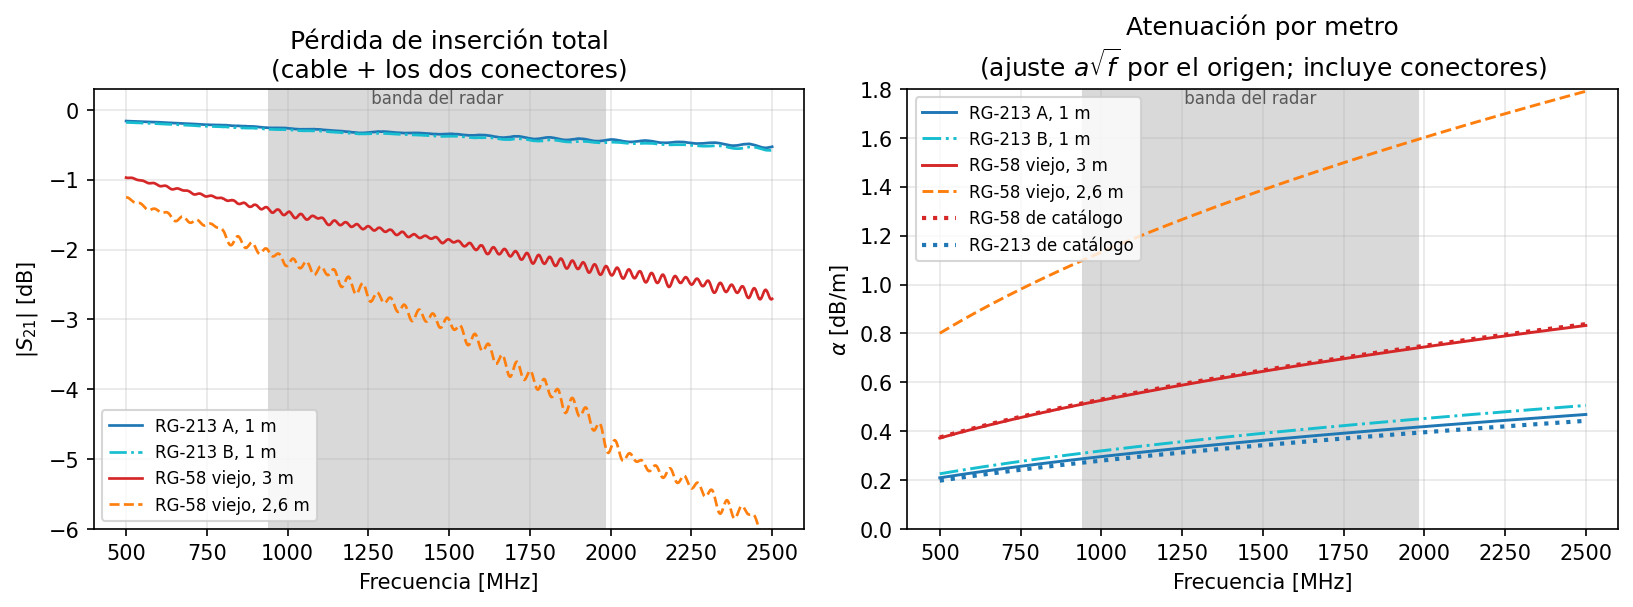
\includegraphics[width=\linewidth]{figuras/cables/cables_insercion.png}
  \caption{Pérdida de inserción medida con el VNA. Izquierda: pérdida
    total $|S_{21}|$ tal como se mide, cable más sus dos conectores; el
    rizado fino es la interferencia entre los dos conectores. Derecha:
    atenuación por metro ajustada como $a\sqrt{f}$ por el origen, con
    los valores de catálogo superpuestos en punteado. Los dos RG-213 y
    el RG-58 de $3\,\text{m}$ caen sobre sus referencias de catálogo;
    el RG-58 de $2{,}6\,\text{m}$ queda al doble y, a la izquierda, se
    curva hacia abajo en vez de seguir la raíz.}
  \label{fig:cables_s21}
\end{figure}

\textbf{Por qué el ajuste se fuerza por el origen.} Se probó primero
con $a\sqrt{f} + b$, esperando que el término constante $b$ se quedara
con lo que no depende del largo: los dos conectores y el desadaptado.
No funciona. En una banda de apenas $500$ a $2500\,\text{MHz}$,
$\sqrt{f}$ y la constante están demasiado correlacionadas para
separarse, y $b$ salió \emph{negativo} en los cuatro cables
($-0{,}15$ en los dos RG-213, $-0{,}48$ en el RG-58 de $3\,\text{m}$ y
$-3{,}43\,\text{dB}$ en el de $2{,}6\,\text{m}$), lo que como pérdida de conector no
existe: lo que hacía era absorber la desviación respecto de la raíz e
inflarle $a$ al cable. Forzado por el origen los números caen sobre el
catálogo, como se ve en la figura. Queda dicho lo que el ajuste
\textbf{no} hace: la pérdida de los conectores sigue adentro de
$\alpha$, repartida en el largo del cable. Separarla exige medir dos
largos del mismo tipo de cable y restar.

\begin{table}[H]
  \centering
  \caption{Atenuación medida y de catálogo en la banda del radar. Los
    dos RG-213 difieren entre sí un $8$\,\% y quedan a menos de un
    $15$\,\% del catálogo con los conectores incluidos. El cable de
    $2{,}6\,\text{m}$ atenúa el doble que su gemelo de $3\,\text{m}$,
    siendo el mismo tipo de cable.}
  \label{tab:cables_alfa}
  \begin{tabular}{lcccc}
    \toprule
    \textbf{Cable} & $\bm{\alpha}$ \textbf{@} $\bm{1\,}$\textbf{GHz}
    & \textbf{Catálogo} & $\bm{\alpha}$ \textbf{@} $\bm{1{,}46\,}$\textbf{GHz}
    & \textbf{Total @} $\bm{1{,}46\,}$\textbf{GHz} \\
    \midrule
    RG-213 A, $1\,\text{m}$          & $0{,}296$ dB/m & $0{,}28$ dB/m & $0{,}358$ dB/m & $0{,}36$ dB \\
    RG-213 B, $1\,\text{m}$          & $0{,}320$ dB/m & $0{,}28$ dB/m & $0{,}387$ dB/m & $0{,}39$ dB \\
    RG-58 viejo, $3\,\text{m}$       & $0{,}527$ dB/m & $0{,}53$ dB/m & $0{,}637$ dB/m & $1{,}91$ dB \\
    RG-58 viejo, $2{,}6\,\text{m}$   & $1{,}132$ dB/m & $0{,}53$ dB/m & $1{,}369$ dB/m & $3{,}56$ dB \\
    \bottomrule
  \end{tabular}
\end{table}

\textbf{El cable de $2{,}6\,\text{m}$ se supone en mal estado}, por las
tres razones que se reúnen en la Sección~\ref{sub:cables_defectuoso}.
Se lo grafica porque es uno de los dos cables que efectivamente
estuvieron en el banco, pero no se lo usa para caracterizar al RG-58:
para eso sirve el de $3\,\text{m}$, que sí se comporta como su hoja de
datos.

\subsection{Resultados: adaptación y pérdida de retorno}
\label{sub:cables_s11_medido}

\begin{figure}[H]
  \centering
  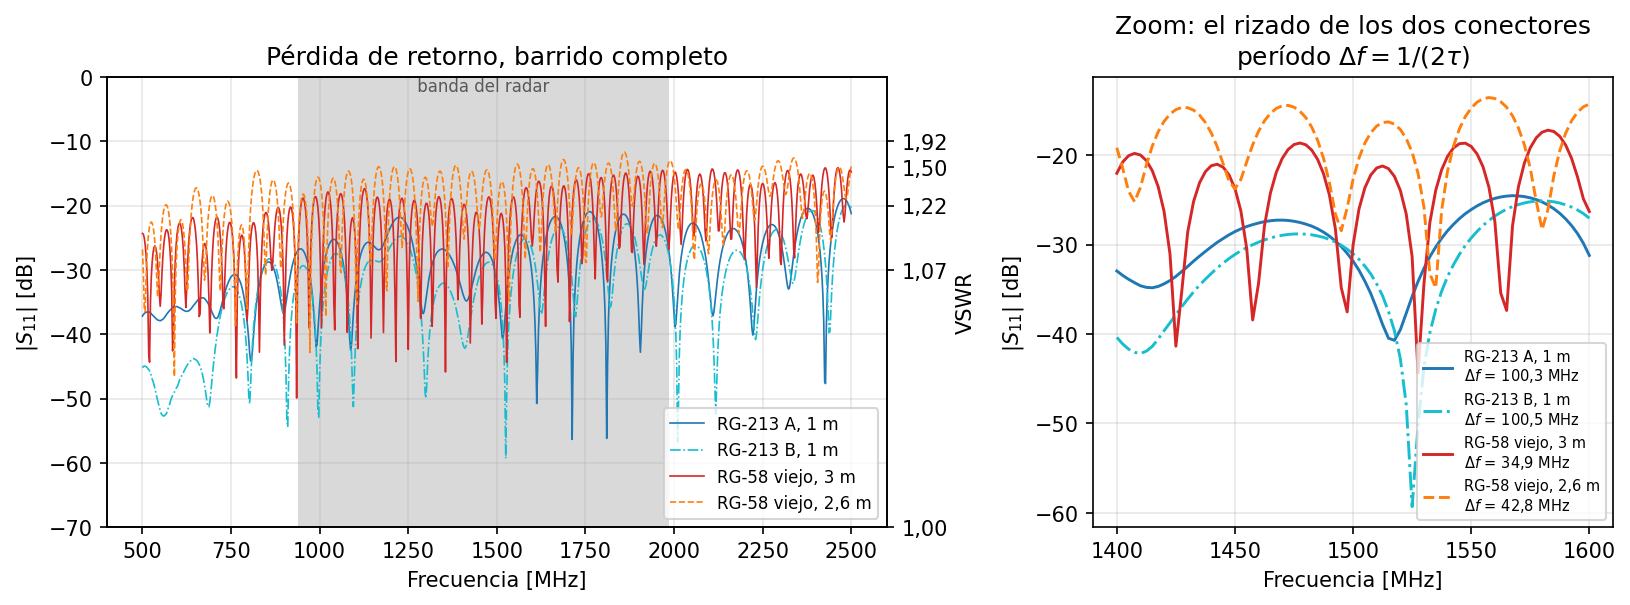
\includegraphics[width=\linewidth]{figuras/cables/cables_retorno.png}
  \caption{Pérdida de retorno. Izquierda: $|S_{11}|$ en todo el
    barrido, con la escala de VSWR equivalente a la derecha y la banda
    del radar sombreada. Derecha: zoom de $1400$ a $1600\,\text{MHz}$.
    El rizado no es ruido: es la interferencia entre las reflexiones de
    los dos conectores, y su período vale $\Delta f = 1/(2\tau)$, con
    $\tau$ el retardo medido de la fase. A cable más largo, rizado más
    apretado.}
  \label{fig:cables_s11}
\end{figure}

Los dos RG-213 quedan por debajo de VSWR $1{,}20$ en toda la banda del
radar, y el RG-58 de $3\,\text{m}$ por debajo de $1{,}46$. El de
$2{,}6\,\text{m}$ llega a $1{,}71$ ($|S_{11}| = -11{,}7\,\text{dB}$):
es el peor de los cuatro, aunque sigue sin ser un desadaptado grave.

Los períodos del zoom cierran con el retardo que se mide por otro
camino en la sección siguiente: $100\,\text{MHz}$ en los cables de
$1\,\text{m}$ corresponden a $\tau = 5{,}0\,\text{ns}$, y
$34{,}9\,\text{MHz}$ en el de $3\,\text{m}$ a $14{,}3\,\text{ns}$.
\textbf{El rizado contiene el retardo}, y fue lo que permitió estimarlo
en la primera tanda de mediciones, cuando todavía no se tenía la fase.

\subsection{Resultados: retardo y VF real}
\label{sub:cables_retardo_medido}

Con la fase de $S_{21}$ el retardo se mide directo: un cable ideal es
un retardo puro, $S_{21} = |S_{21}|\,e^{-j\omega\tau}$, así que la
fase desenrollada es una recta en $\omega$ y su pendiente, cambiada de
signo, es $\tau$. Se ajustó esa recta sobre todo el barrido, de $500$ a
$2500\,\text{MHz}$. El desvío rms de la fase respecto de la recta
indica cuánto se aparta el cable de un retardo puro, y resulta útil
para diagnosticarlo.

Con $S_{11}$ en magnitud y fase se puede además calcular la
\textbf{respuesta al impulso} del cable: la transformada inversa de
$S_{11}(f)$ muestra cada discontinuidad como un pico en su tiempo de
ida y vuelta. Es el modo ``dominio del tiempo'' de un VNA, hecho
fuera del equipo. Como el barrido es de banda pasante ($500$ a
$2500\,\text{MHz}$) y se aplica ventana de Hann, la resolución es de
un poco más de $1/BW = 0{,}5\,\text{ns}$ de ida y vuelta.

\begin{figure}[H]
  \centering
  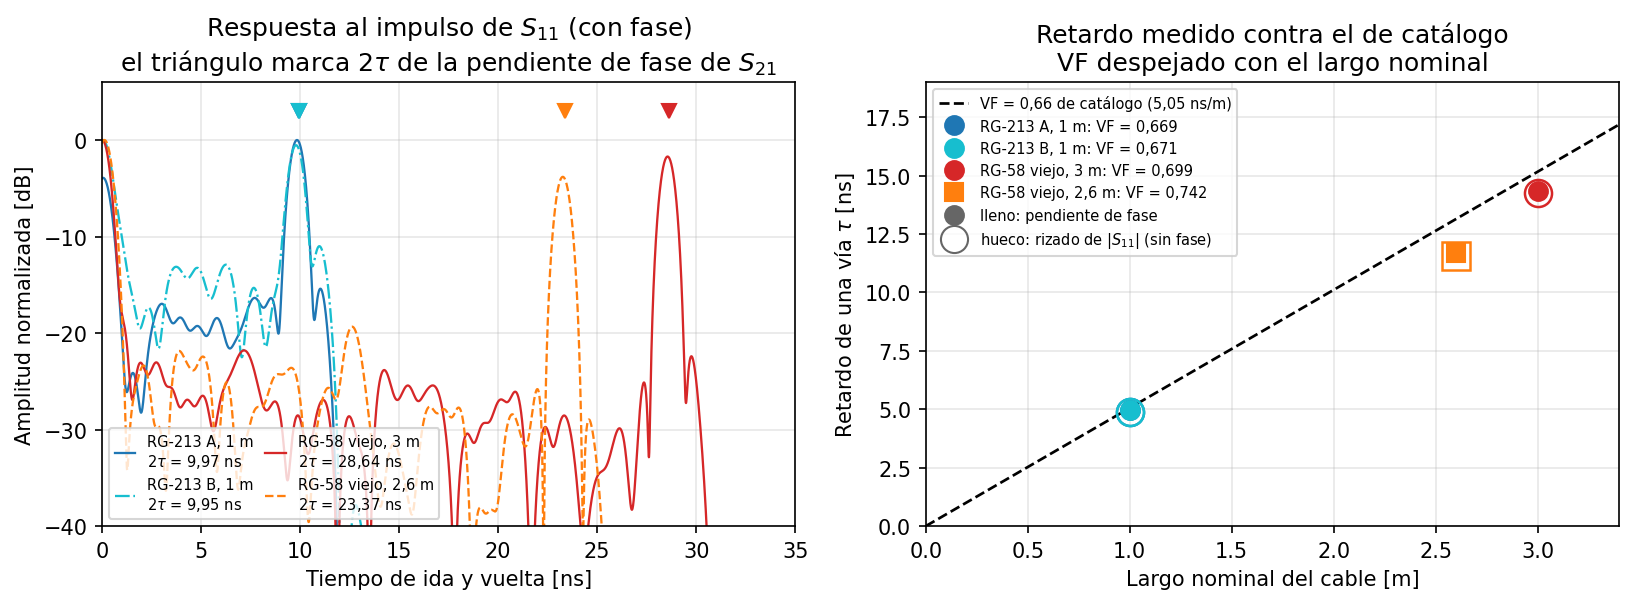
\includegraphics[width=\linewidth]{figuras/cables/cables_tiempo.png}
  \caption{Izquierda: respuesta al impulso de $S_{11}$ complejo, en
    dB respecto del pico mayor. Cada pico es una reflexión, ubicada en
    su tiempo de ida y vuelta; el triángulo marca $2\tau$ tomado de la
    pendiente de fase de $S_{21}$, y coincide con el eco del extremo en
    los cuatro cables. El RG-58 de $2{,}6\,\text{m}$ (naranja) muestra
    además un pico a mitad de camino, en $12{,}6\,\text{ns}$.
    Derecha: retardo de una vía contra el largo nominal. Los símbolos
    llenos son la pendiente de fase y los huecos, el rizado de
    $|S_{11}|$; la recta es el VF $0{,}66$ de catálogo.}
  \label{fig:cables_tiempo}
\end{figure}

\textbf{Los dos métodos coinciden.} El eco del extremo cae exactamente
donde lo pone la pendiente de fase, obtenida de otro parámetro
($S_{21}$ y no $S_{11}$), y el retardo del rizado difiere del de fase
entre $0{,}05$ y $0{,}12\,\text{ns}$, siempre dentro de la resolución
de $\pm0{,}25\,\text{ns}$ que se le había asignado a ese método. La
diferencia está en la precisión: el ajuste de fase usa las $801$
muestras y no depende de dónde cae un bin de la FFT.

\begin{table}[H]
  \centering
  \caption{Retardo medido de la pendiente de fase de $S_{21}$. Las
    columnas de $L$ y VF son dos lecturas del mismo dato: fijando el VF
    de catálogo se despeja el largo eléctrico, y fijando el largo
    nominal se despeja el VF. La última columna es el desvío rms de la
    fase respecto de un retardo puro.}
  \label{tab:cables_retardo}
  \small\setlength{\tabcolsep}{4pt}
  \begin{tabular}{lccccc}
    \toprule
    \textbf{Cable} & $\bm{\tau}$ & \textbf{ns/m}
    & $\bm{L}$ \textbf{si VF} $\bm{=0{,}66}$ & \textbf{VF si} $\bm{L}$ \textbf{nominal}
    & \textbf{Desvío de fase} \\
    \midrule
    RG-213 A, $1\,\text{m}$        & $4{,}983$ ns  & $4{,}98$ & $0{,}99$ m & $0{,}669$ & $0{,}09^\circ$ \\
    RG-213 B, $1\,\text{m}$        & $4{,}975$ ns  & $4{,}98$ & $0{,}98$ m & $0{,}671$ & $0{,}08^\circ$ \\
    RG-58 viejo, $3\,\text{m}$     & $14{,}319$ ns & $4{,}77$ & $2{,}83$ m & $0{,}699$ & $0{,}37^\circ$ \\
    RG-58 viejo, $2{,}6\,\text{m}$ & $11{,}686$ ns & $4{,}49$ & $2{,}31$ m & $0{,}742$ & $1{,}78^\circ$ \\
    \bottomrule
  \end{tabular}
\end{table}

\textbf{Los RG-213 confirman el catálogo.} Los dos dan VF $0{,}67$, a
$1{,}5$\,\% del $0{,}66$ nominal, y difieren entre sí apenas
$8\,\text{ps}$. Una diferencia de $1{,}5$\,\% en un cable de
$1\,\text{m}$ son $1{,}5\,\text{cm}$ de largo, que es del orden del
error de medir el cable con cinta y de dónde se toma el plano de
referencia de los conectores. Con fase, el primer valor que se había
despejado del rizado ($0{,}684$) resulta ser error del método.

\textbf{Los RG-58 viejos dan más rápidos}: $0{,}699$ el de
$3\,\text{m}$ y $0{,}742$ el de $2{,}6\,\text{m}$. Medidos con cinta,
los dos cables tienen aproximadamente su largo nominal, así que la
diferencia no se explica por el largo: para ajustarse al catálogo, el
de $3\,\text{m}$ tendría que medir unos $17\,\text{cm}$ menos. En ese
cable es probable que el dieléctrico no sea exactamente el del RG-58
de catálogo. El
valor del de $2{,}6\,\text{m}$ no es físico para polietileno sólido y
se trata en la sección siguiente. Aun así, \textbf{todos los cálculos
de diseño de este capítulo siguen usando el VF nominal $0{,}66$}: es
el valor que se conoce sin medir, y el offset real del banco se corrige
igual con la calibración de la Sección~\ref{sec:cables_calibracion}.

\subsection{El cable de $2{,}6\,\text{m}$: por qué se lo supone en mal estado}
\label{sub:cables_defectuoso}

El cable de $2{,}6\,\text{m}$ es uno de los dos que estuvieron en el
banco, del lado de RX, y se sospechaba de él antes de medirlo. Las
mediciones muestran tres indicios independientes, cada uno en un
parámetro distinto:

\begin{enumerate}
  \item \textbf{Atenúa el doble de lo que le corresponde, y no con la
    forma de un cable.} Da $1{,}13\,\text{dB/m}$ a $1\,\text{GHz}$
    contra los $0{,}53$ del catálogo y los $0{,}527$ que midió su
    gemelo de $3\,\text{m}$ (Tabla~\ref{tab:cables_alfa}). Aun siendo
    $40\,\text{cm}$ más corto, pierde $3{,}56\,\text{dB}$ en el centro
    de la banda contra $1{,}91$. Además, la pérdida no crece como
    $\sqrt{f}$: en la Figura~\ref{fig:cables_s21} la curva se dobla
    hacia abajo, y el ajuste libre $a\sqrt{f}+b$ necesita un término
    constante de $-3{,}43\,\text{dB}$ para seguirla, siete veces el del
    RG-58 sano. El efecto pelicular y el dieléctrico por sí solos
    no dan esa forma.
  \item \textbf{Es el peor adaptado de los cuatro.} $|S_{11}|$ llega a
    $-11{,}7\,\text{dB}$ (VSWR $1{,}71$) en la banda del radar, contra
    $-14{,}5\,\text{dB}$ del RG-58 de $3\,\text{m}$ y
    $-21\,\text{dB}$ de los RG-213 (Figura~\ref{fig:cables_s11}).
    Refleja más en sus extremos, que es lo que se espera de un conector
    mal armado o flojo.
  \item \textbf{Su retardo no es el de un cable sano.} La fase de
    $S_{21}$ se aparta $1{,}78^\circ$ rms de un retardo puro, cinco
    veces más que el RG-58 de $3\,\text{m}$ y veinte veces más que los
    RG-213 (Tabla~\ref{tab:cables_retardo}). El VF que se despeja,
    $0{,}742$, no es posible en polietileno sólido. Y en la respuesta
    al impulso (Figura~\ref{fig:cables_tiempo}) aparece una reflexión
    \emph{dentro} del cable, unos $15\,\text{dB}$ por debajo del eco
    del extremo. Esa reflexión se ve desde los dos puertos: en
    $12{,}63\,\text{ns}$ desde el puerto~1 y en $10{,}77\,\text{ns}$
    desde el puerto~2. Las dos lecturas suman $23{,}40\,\text{ns}$,
    igual a los $2\tau = 23{,}37\,\text{ns}$ del cable, así que no es
    un artefacto de la transformada: es un punto físico, a unos
    $1{,}4\,\text{m}$ de un extremo y $1{,}2\,\text{m}$ del otro.
\end{enumerate}

Los dos primeros indicios son compatibles con un conector en mal
estado, que era la hipótesis inicial. El tercero sugiere que el daño
no está solo en los extremos: una discontinuidad a mitad del cable
puede ser un aplastamiento, un doblez por debajo del radio mínimo o un
empalme. Conviene no sobreinterpretarlo. El RG-58 de $3\,\text{m}$,
que en todo lo demás se comporta bien, muestra un par de reflexiones
internas del mismo tipo, unos $5\,\text{dB}$ más débiles respecto de su
propio eco del extremo. Además, una reflexión chica no alcanza para
explicar por sí sola los $1{,}9\,\text{dB}$ que pierde de más en el
centro de la banda: un daño con pérdida puede reflejar poco.

La conclusión práctica es la misma en cualquier caso: \textbf{el cable
de $2{,}6\,\text{m}$ no representa al RG-58} y no conviene volver a
usarlo en el banco. Que el defecto esté en un conector o en el cable
solo decide si vale la pena rearmarlo.

\subsection{Consecuencias para el radar}
\label{sub:cables_impacto}

\begin{figure}[H]
  \centering
  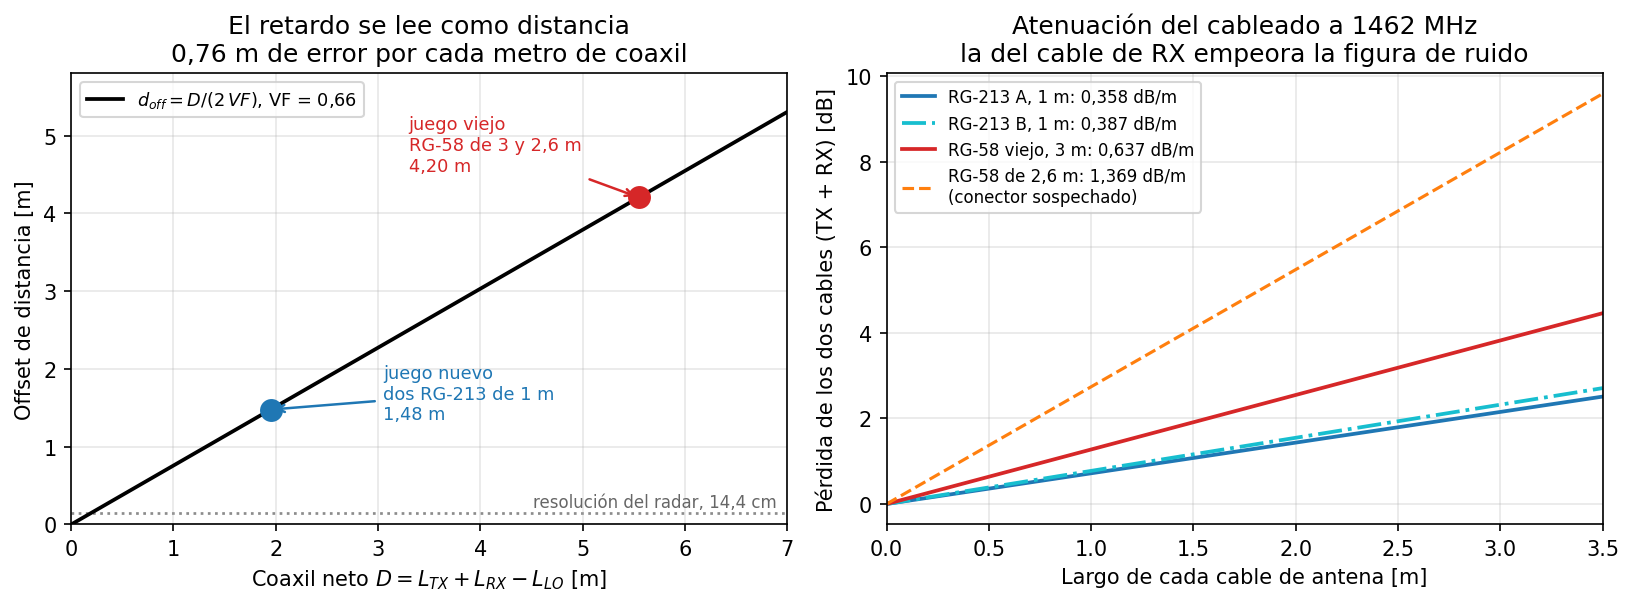
\includegraphics[width=\linewidth]{figuras/cables/cables_impacto.png}
  \caption{Lo que el cableado le cuesta al radar. Izquierda: offset de
    distancia $d_\text{offset} = D/(2\,\text{VF})$ con el VF $0{,}66$
    de catálogo, según el coaxil neto $D$, con los dos juegos de cables
    marcados. Derecha: pérdida de un par de cables (TX más RX) en el
    centro de la banda, $1462\,\text{MHz}$, en función del largo de
    cada uno, con la atenuación por metro medida en cada cable. La
    recta del RG-58 de $2{,}6\,\text{m}$ es la del cable dañado
    (Sección~\ref{sub:cables_defectuoso}), no la de un RG-58.}
  \label{fig:cables_impacto}
\end{figure}

Los dos costos se leen por separado. En \textbf{retardo}, cambiar los
RG-58 de $3$ y $2{,}6\,\text{m}$ por los dos RG-213 de $1\,\text{m}$
baja el offset de $4{,}20\,\text{m}$ a $1{,}48\,\text{m}$ con los
valores de catálogo, o de $3{,}86\,\text{m}$ a $1{,}45\,\text{m}$ con
los retardos medidos (Tabla~\ref{tab:cables_teoria_practica}). Sigue siendo
diez veces la resolución de $14{,}4\,\text{cm}$, así que \textbf{acortar
los cables no reemplaza a la calibración} de la
Sección~\ref{sec:cables_calibracion}: solo la vuelve una corrección más
chica. Lo único que anula el offset de raíz es emparejar el LO
(Tabla~\ref{tab:cables_nuevo_offset}).

En \textbf{atenuación}, el par original costaba $5{,}5\,\text{dB}$ a
$1{,}46\,\text{GHz}$ contra los $0{,}75\,\text{dB}$ del par nuevo. De
esos $4{,}7\,\text{dB}$ recuperados, sin embargo, solo una parte es
mérito del RG-213: dos RG-58 sanos de esos largos habrían costado
$3{,}6\,\text{dB}$, así que $1{,}9\,\text{dB}$ los estaba perdiendo el
cable de $2{,}6\,\text{m}$ en mal estado y se habrían recuperado con
solo reemplazarlo. La mitad de la mejora cae delante del
LNA, donde se descuenta uno a uno de la figura de ruido de toda la
cadena.

\subsection{Resultados: espectro de batido con blanco fijo}

\begin{figure}[H]
  \centering
  % TODO: dos capturas del panel de FFT de vivo.py (o
  % graficar_captura.py), mismo blanco y misma distancia, una con los
  % cables originales y otra con los nuevos. Señalar en cada una la
  % posición del pico, su ancho a -3 dB y el piso de ruido.
  % \includegraphics[width=0.48\linewidth]{figuras/cables/espectro_cable_original.png}
  % \includegraphics[width=0.48\linewidth]{figuras/cables/espectro_cable_nuevo.png}
  \fbox{\parbox{0.9\linewidth}{\centering\vspace{3cm}
    \textit{Pendiente: espectro de batido (\texttt{vivo.py}), mismo
    blanco y misma distancia, cable original vs.\ cable nuevo.
    Indicar posición del pico, ancho a $-3\,\text{dB}$ y piso de
    ruido.}\vspace{3cm}}}
  \caption{Efecto del cable sobre el espectro de batido: posición del
    pico (retardo), y forma/piso de ruido (pérdida y SNR).}
  \label{fig:cables_espectro_template}
\end{figure}

Dos efectos de los cables se superponen en esta comparación y conviene
no confundirlos: acortar el cable \textbf{corre el pico} (menos
retardo, Sección~\ref{sec:cables_offset}) y, si además reduce la
atenuación, \textbf{puede subir el piso de SNR} (menos pérdida de
inserción antes del LNA, Sección~\ref{sec:cables_perdidas}). Son
efectos independientes: el primero se lee en el eje de frecuencia
(dónde cae el pico) y el segundo en el eje de amplitud (cuánto se
levanta el pico sobre el piso de ruido). La comparación debe reportar
ambos por separado, no un único número.

\subsection{Comparación teoría vs.\ práctica: tabla resumen}

\begin{table}[H]
  \centering
  \caption{Resumen comparativo entre el valor teórico (predicho por las
    ecuaciones de este capítulo, a partir de las longitudes nominales
    y el $\text{VF}$ de catálogo) y el valor medido con el VNA a partir
    de la fase de $S_{21}$, para ambos juegos de cables.}
  \label{tab:cables_teoria_practica}
  \small\setlength{\tabcolsep}{4pt}
  \begin{tabular}{lcccc}
    \toprule
    & \multicolumn{2}{c}{\textbf{Juego original (2 RG-58)}}
    & \multicolumn{2}{c}{\textbf{Juego nuevo (2 RG-213)}} \\
    \cmidrule(lr){2-3}\cmidrule(lr){4-5}
    & Teoría & Medido & Teoría & Medido \\
    \midrule
    VF                                        & $0{,}66$\textsuperscript{*} & $0{,}70$ / $0{,}74$\textsuperscript{\dag} & $0{,}66$\textsuperscript{*} & $0{,}67$\textsuperscript{\dag} \\
    $\tau_\text{TX}+\tau_\text{RX}$ {[}ns{]}  & $28{,}3$ & $26{,}0$ & $10{,}1$ & $9{,}96$ \\
    $L_\text{TX}+L_\text{RX}$ {[}m{]}         & $5{,}60$ & $5{,}15$ & $2{,}00$ & $1{,}97$ \\
    $d_\text{offset}$ {[}m{]}\textsuperscript{\S} & $4{,}20$ & $\bm{3{,}86}$ & $1{,}48$ & $\bm{1{,}45}$ \\
    Atenuación del par @ $1{,}5\,\text{GHz}$ {[}dB{]} & $3{,}64$ & $5{,}47$\textsuperscript{\ddag} & $0{,}69$ & $0{,}75$ \\
    \bottomrule
  \end{tabular}

  \vspace{4pt}
  \begin{minipage}{0.92\linewidth}\footnotesize
    \textsuperscript{*}Valor nominal de catálogo
    (Tabla~\ref{tab:vf_cables}), que es el que se usa en todos los
    cálculos de diseño de este capítulo.

    \textsuperscript{\dag}Despejado del retardo de fase suponiendo el
    largo nominal de cada cable, que coincide aproximadamente con el
    medido con cinta; en el juego original, $3\,\text{m}$ y
    $2{,}6\,\text{m}$ por separado. Para diseño se sigue usando el
    nominal --- ver Sección~\ref{sub:cables_retardo_medido}.

    \textsuperscript{\ddag}Incluye el cable de $2{,}6\,\text{m}$ en mal
    estado (Sección~\ref{sub:cables_defectuoso}), que por sí solo
    aporta $3{,}56\,\text{dB}$ de los $5{,}47$. Dos RG-58 sanos de esos
    largos habrían costado $3{,}6\,\text{dB}$, extrapolando el $\alpha$
    medido del cable de $3\,\text{m}$.

    \textsuperscript{\S}El camino del LO es una conexión directa de
    $\approx 5\,\text{cm}$, que aporta $0{,}25\,\text{ns}$: se lo resta
    en las dos columnas, pero equivale a $3{,}8\,\text{cm}$ y no cambia
    ninguna conclusión. La columna ``medido'' no depende, entonces, de
    ningún valor supuesto.
  \end{minipage}
\end{table}

\textbf{El offset medido no depende de suponer nada}, y eso lo hace el
número más sólido de la tabla: sale de multiplicar el retardo de fase
por $c_0/2$, sin pasar por el factor de velocidad ni por el largo de
cinta métrica. En el juego nuevo da $1{,}45\,\text{m}$ contra
$1{,}48\,\text{m}$ de la ecuación~\eqref{eq:d_offset}, un $2$\,\% de
diferencia. En el original da $3{,}86\,\text{m}$ contra $4{,}20$, un
$8$\,\% menos.

El del juego original cierra además con una estimación completamente
independiente, hecha en el banco antes de tener el VNA: con
$T_c = 80\,\text{ms}$, una placa a $1\,\text{m}$ daba algo más de
$800\,\text{Hz}$, de donde el offset resultaba
$\approx 3{,}6\,\text{m}$. Tres caminos que no comparten ni el
instrumento ni el método ---la ecuación, el VNA y el propio radar---
caen dentro de un $15$\,\%, con los dos valores experimentales por
debajo del teórico y a un $7$\,\% entre sí.

La diferencia entre los dos juegos está en los cables, no en la
ecuación. Los RG-213 miden el VF de catálogo
(Tabla~\ref{tab:cables_retardo}), y con ellos teoría y medición
coinciden. Los RG-58 viejos miden más rápidos que el nominal, y el de
$2{,}6\,\text{m}$ bastante más, por el daño descripto en la
Sección~\ref{sub:cables_defectuoso}. Por eso con ese juego la teoría
queda alta. El largo no es la causa: medidos con cinta, los cables
tienen aproximadamente su largo nominal.

%============================================================
%  APÉNDICES
%============================================================
\appendix

%============================================================
\chapter{La transformada chirp-Z (CZT) — trabajo futuro}
\label{ap:czt}
%============================================================

\textit{Este capítulo queda como apéndice de referencia teórica para
una etapa posterior de la tesis. Todavía no se implementó ni se
validó experimentalmente sobre el banco de pruebas: la separación de
reflexiones cercanas (espesor de capa) se está resolviendo por ahora
con la FFT estándar. Se deja documentado acá porque es la técnica que
se evaluará más adelante para mejorar esa resolución, no porque el
resto de la tesis dependa de ella.}

\section{Limitación de resolución del FFT}
\label{sec:limitacion_fft}

La resolución frecuencial de la DFT calculada sobre $N$ muestras a
frecuencia de muestreo $f_s$ es:

\begin{equation}
  \Delta f_\text{FFT} = \frac{f_s}{N}\quad[\text{Hz}].
  \label{eq:res_fft}
\end{equation}

En el sistema de referencia~\cite{Huang2022}: $f_s = 100\,\text{Hz}$,
$N = f_s \cdot T_c = 30$ muestras, lo que da:

\begin{equation*}
  \Delta f_\text{FFT} = \frac{100}{30} \approx 3{,}33\,\text{Hz/bin}.
\end{equation*}

Si la diferencia real entre los picos es $\Delta f = 4\,\text{Hz}$,
el FFT apenas puede distinguirla, con un error de espesor que puede
superar los $20\,\text{mm}$.

Aumentar $N$ exigiría una mayor frecuencia de muestreo (hardware más
costoso), sin beneficio real dado que las frecuencias IF son bajas
($< 60\,\text{Hz}$). La CZT es una alternativa para resolver este
problema sin modificar el hardware, a evaluar más adelante.

\section{Conceptos fundamentales de la CZT}
\label{sec:czt_teoria}

La transformada-Z de una secuencia $x[n]$ de longitud $N$, evaluada en
$M$ puntos dispuestos sobre un arco del plano complejo, es:

\begin{equation}
  X_\text{CZT}[k] = \sum_{n=0}^{N-1} x[n]\, z_k^{-n},
  \qquad k = 0, 1, \ldots, M-1,
  \label{eq:czt_def}
\end{equation}

con los puntos de evaluación:

\begin{equation}
  z_k = A_0\, W_0^{-k},
  \label{eq:zk}
\end{equation}

donde:

\begin{align}
  A_0 &= e^{\,j\,\omega_\text{start}} = e^{\,j\,2\pi f_\text{start}/f_s}, \label{eq:A0}\\
  W_0 &= e^{-j\,\Delta\omega} = e^{-j\,2\pi(f_\text{end}-f_\text{start})/(f_s(M-1))}. \label{eq:W0}
\end{align}

La resolución espectral resultante es:

\begin{equation}
  \Delta f_\text{CZT} = \frac{f_\text{end} - f_\text{start}}{M-1}\quad[\text{Hz}].
  \label{eq:res_czt}
\end{equation}

\subsection*{Caso especial: CZT $\equiv$ DFT}

Si $A_0 = 1$ y $W_0 = e^{-j2\pi/N}$, la CZT cubre el círculo unitario
completo con $N$ puntos igualmente espaciados y su resultado es
idéntico al DFT estándar. El FFT convencional es un caso particular
de la CZT.

\section{Tabla de parámetros CZT}
\label{sec:tabla_czt}

\begin{table}[H]
  \centering
  \caption{Parámetros de la CZT y su cálculo desde $f_\text{start}$,
  $f_\text{end}$ y $f_s$.}
  \label{tab:czt_params}
  \begin{tabular}{p{1.5cm}p{4.5cm}p{6cm}}
    \toprule
    \textbf{Símbolo} & \textbf{Significado} & \textbf{Cálculo} \\
    \midrule
    $A_0$ & Punto de inicio en el plano $z$
    & $A_0 = e^{\,j\,2\pi f_\text{start}/f_s}$ \\[4pt]
    $W_0$ & Paso entre muestras (módulo~1)
    & $W_0 = e^{-j\,2\pi(f_\text{end}-f_\text{start})/(f_s(M-1))}$ \\[4pt]
    $\Delta\omega$ & Paso angular
    & $\Delta\omega = 2\pi(f_\text{end}-f_\text{start})/(f_s(M-1))$ \\[4pt]
    $M$   & Número de puntos del zoom
    & Elegido por el usuario (potencia de~2 recomendada) \\[4pt]
    $k$   & Índice de salida
    & $k = 0, 1, \ldots, M-1$ \\
    \bottomrule
  \end{tabular}
\end{table}

\section{Implementación eficiente: algoritmo de Bluestein}
\label{sec:bluestein}

El cálculo directo de la ecuación~\eqref{eq:czt_def} tiene complejidad
$\mathcal{O}(N\cdot M)$. El algoritmo de Bluestein reduce esto a
$\mathcal{O}((N+M)\log(N+M))$ mediante la identidad algebraica:

\begin{equation}
  k\cdot n = \frac{n^2}{2} + \frac{k^2}{2} - \frac{(k-n)^2}{2},
\end{equation}

que convierte la suma del CZT en una convolución implementable con FFT.
Los pasos son los siguientes:

\begin{enumerate}
  \item \textbf{Pre-multiplicación:}
    $y[n] = x[n]\cdot A_0^{-n}\cdot W_0^{n^2/2}$.

  \item \textbf{Definición del filtro:}
    \begin{equation*}
      h[k] = W_0^{-k^2/2}, \quad k = 0,\ldots,M-1; \quad
      h[L-N+1\,\ldots\,L-1] = W_0^{-(N-k)^2/2}.
    \end{equation*}

  \item \textbf{Convolución vía FFT:}
    \begin{equation*}
      G = \text{IFFT}\!\bigl(\text{FFT}(y,L)\cdot\text{FFT}(h,L)\bigr),
    \end{equation*}
    donde $L$ es la potencia de 2 más próxima superior a $M+N-1$.

  \item \textbf{Post-multiplicación:}
    $X_\text{CZT}[k] = G[k]\cdot W_0^{k^2/2}$, \quad $k=0,\ldots,M-1$.

  \item \textbf{Eje de frecuencias:}
    \begin{equation}
      f[k] = f_\text{start} + k\cdot\frac{f_\text{end}-f_\text{start}}{M-1}.
      \label{eq:eje_f}
    \end{equation}
\end{enumerate}

\subsection{Ejemplo numérico}
\label{sub:ejemplo_czt}

$N = 30$ muestras, $f_s = 100\,\text{Hz}$, zoom: $f_\text{start}=3\,\text{Hz}$,
$f_\text{end}=15\,\text{Hz}$, $M=512$ puntos.

\begin{table}[H]
  \centering
  \caption{Cálculo de los parámetros CZT para el ejemplo de referencia.}
  \label{tab:ejemplo_czt}
  \begin{tabular}{ll}
    \toprule
    \textbf{Cálculo} & \textbf{Resultado} \\
    \midrule
    $\omega_\text{start}$ & $2\pi\times3/100 = 0{,}18850\,\text{rad}$ \\
    $\omega_\text{end}$   & $2\pi\times15/100 = 0{,}94248\,\text{rad}$ \\
    $\Delta\omega$         & $(0{,}94248-0{,}18850)/511 = 0{,}001476\,\text{rad/muestra}$ \\
    $\Delta f_\text{CZT}$ & $(15-3)/511 \approx 0{,}0235\,\text{Hz/bin}$ \\
    $\Delta f_\text{FFT}$ & $100/30 \approx 3{,}33\,\text{Hz/bin}$ (142$\times$ peor) \\
    $A_0$                 & $\cos(0{,}18850)+j\sin(0{,}18850)$ \\
    $W_0$                 & $e^{-j\,0{,}001476}$ \\
    $L$                   & $2^{\lceil\log_2(512+30-1)\rceil} = 2^{10} = 1024$ \\
    \bottomrule
  \end{tabular}
\end{table}

\section{Guía de selección de parámetros}
\label{sec:guia_params}

\subsection{Rango de zoom [$f_\text{start}$, $f_\text{end}$]}

\begin{enumerate}
  \item Calcular el FFT completo para identificar la región de interés.
  \item Estimar el rango esperado de $\Delta f$ con la inversa de la
    ecuación~\eqref{eq:espesor}:
    \begin{equation}
      \Delta f_\text{max} = \frac{4\sqrt{\varepsilon_r}\,B\,h_\text{max}}{T_c\,c},
      \quad
      \Delta f_\text{min} = \frac{4\sqrt{\varepsilon_r}\,B\,h_\text{min}}{T_c\,c}.
    \end{equation}
  \item Agregar un margen del 30–50\% a cada lado.
\end{enumerate}

\subsection{Número de puntos $M$}

\begin{table}[H]
  \centering
  \caption{Resolución CZT para distintos valores de $M$ (rango de
  zoom de 12\,Hz).}
  \label{tab:M_resolucion}
  \begin{tabular}{ccl}
    \toprule
    $M$ & $\Delta f_\text{CZT}$ & \textbf{Uso recomendado} \\
    \midrule
    128  & $\approx 0{,}094\,\text{Hz}$ & Exploración rápida, capas gruesas ($>15\,\text{cm}$) \\
    512  & $\approx 0{,}024\,\text{Hz}$ & Balance calidad/velocidad, uso general \\
    2048 & $\approx 0{,}006\,\text{Hz}$ & Alta precisión, capas delgadas ($<5\,\text{cm}$) \\
    8192 & $\approx 0{,}0015\,\text{Hz}$ & Máxima resolución, verificación crítica \\
    \bottomrule
  \end{tabular}
\end{table}

\textit{Regla práctica:} $\Delta f_\text{CZT} < \Delta f_\text{real}/5$.

\section{Flujo completo del algoritmo (a futuro)}
\label{sec:flujo_czt}

\begin{table}[H]
  \centering
  \caption{Resumen del flujo de procesamiento GPR FMCW con CZT, propuesto para cuando se implemente.}
  \label{tab:flujo}
  \begin{tabular}{clp{7cm}}
    \toprule
    \textbf{\#} & \textbf{Etapa} & \textbf{Descripción} \\
    \midrule
    1 & Emisión del chirp
    & El radar barre de $f_c - B/2$ a $f_c + B/2$ en tiempo $T_c/2$
    (media triangular). \\
    2 & Reflexiones
    & $R_1$ y $R_2$ llegan con retardos $\tau_1$, $\tau_2$. \\
    3 & Mezcla (\textit{mixer})
    & $s_\text{tx}\times s_\text{rx}$ + LPF $\rightarrow$ señal IF con
    $f_1 = S\tau_1$ y $f_2 = S\tau_2$. \\
    4 & Muestreo IF
    & Se digitaliza la señal IF con $N$ muestras a $f_s\,\text{Hz}$. \\
    5 & FFT (referencia)
    & Espectro de baja resolución; puede no separar $f_1$ de $f_2$. \\
    6 & Definir zoom CZT
    & Elegir $[f_\text{start}, f_\text{end}]$ y $M$. \\
    7 & Calcular $A_0$, $W_0$, $\Delta\omega$
    & Ec.~\eqref{eq:A0}--\eqref{eq:W0}. \\
    8 & Bluestein
    & Pre-mult. $\to$ convolución FFT $\to$ post-mult. $\to$ magnitud. \\
    9 & Detección de picos
    & Identificar $f_1$ y $f_2$ en el espectro CZT. \\
    10 & Calcular espesor
    & $\Delta f = f_2 - f_1$ $\rightarrow$ ec.~\eqref{eq:espesor}. \\
    \bottomrule
  \end{tabular}
\end{table}

%============================================================
%  BIBLIOGRAFÍA
%============================================================
\printbibliography[heading=bibintoc, title={Referencias}]

\end{document}
